\documentclass[a4paper,11pt]{article}
\usepackage[T1]{fontenc}
\usepackage[utf8]{inputenc}
\usepackage{lmodern}
\usepackage{textcomp}
\usepackage{amssymb}
\usepackage[margin=1.5cm]{geometry}
\usepackage{lscape}

\title{HICF1 -  Final Report v6}
\author{Dr. Susanne Weller}
\date{\today}

\usepackage{Sweave}
\begin{document}
\Sconcordance{concordance:HICF1_Finalreportv6.tex:HICF1_Finalreportv6.Rnw:%
1 13 1 1 0 18 1 1 20 1 37 1 4 26 0 1 2 1 29 1 2 13 1 1 45 1 1 1 6 36 0 %
1 2 1 6 36 0 1 2 5 1 1 17 1 6 36 0 1 2 2 1 1 41 1 3 7 1 1 57 1 4 30 0 1 %
2 2 1 1 36 1 4 19 0 1 2 13 1 1 13 1 2 1 13 1 2 1 13 1 2 1 12 1 3 1 12 1 %
3 1 12 1 3 1 12 1 3 1 1 1 50 1 2 1 6 1 4 18 0 1 2 92 1 1 17 1 2 1 6 1 %
10 1 2 2 1 1 10 1 2 2 1 1 6 1 4 28 0 3 2 1 4 2 2 1 1 1 4 2 2 1 1 1 4 2 %
2 1 1 1 4 2 2 1 1 1 4 2 2 3 1 1 35 1 12 1 2 1 12 1 2 1 12 1 2 1 4 27 0 %
1 2 1 31 1 4 15 0 1 2 3 1 1 13 1 2 2 1}


\maketitle
\tableofcontents

\section{Methods and Programmes used}
\emph{This can go into a paper:}\\
Statistical analysis was carried out using the programme R (version 3.0.1). Survival data was analysed using the additional package "survival" (version 2.37-7). The code for this analysis is publicly available on github:
https://github.com/Suska/HICF1\\
\emph{citation:}\\
R Core Team (2013). R: A language and environment for statistical computing. R Foundation for Statistical Computing, Vienna, Austria. URL http://www.R-project.org/.

\section{Univariate Analysis}
\emph{This can go into a paper:}\\
Univariate analysis was done using Fisher's Exact test for binary genetic variables and wilcoxon signed rank test for continuous variables (Number of CNAs and Subclones). Correction for multiple testing was done using False Discovery Rate.\\
\emph{citation:}\\
Benjamini, Y., and Hochberg, Y. (1995). Controlling the false discovery rate: a practical and powerful approach to multiple testing. Journal of the Royal Statistical Society Series B, 57, 289–300.

\emph{\\Note that TP53\_mut are only mutation with >5\%VAF! Univariate p-values change dramatically if you add more variables, this is due to the multiple testing problem.}

% Table created by stargazer v.5.1 by Marek Hlavac, Harvard University. E-mail: hlavac at fas.harvard.edu
% Date and time: Tue, Sep 30, 2014 - 08:53:01
\begin{table}[!htbp] \centering 
  \caption{Univariate Analysis against MRD outcome} 
  \label{} 
\tiny 
\begin{tabular}{@{\extracolsep{0p}} ccccccccc} 
\\[-1.8ex]\hline 
\hline \\[-1.8ex] 
 & p & sig & corr.p & sig.corr & MRDpos\_0 & MRDneg\_0 & MRDpos\_1 & MRDneg\_1 \\ 
\hline \\[-1.8ex] 
ATM\_bi & $0.004$ & \textasteriskcentered \textasteriskcentered  & $0.011$ & \textasteriskcentered  & 41\% & 48\% & 8\% & 2\% \\ 
ATM\_del & $0.001$ & \textasteriskcentered \textasteriskcentered \textasteriskcentered  & $0.005$ & \textasteriskcentered \textasteriskcentered  & 36\% & 46\% & 13\% & 5\% \\ 
ATM\_mono & $0.502$ & n.s. & $0.554$ & n.s. & 45\% & 45\% & 4\% & 6\% \\ 
BIRC3\_bi & $0.365$ & n.s. & $0.465$ & n.s. & 48\% & 50\% & 1\% & 0\% \\ 
BIRC3\_del & $0.002$ & \textasteriskcentered \textasteriskcentered  & $0.007$ & \textasteriskcentered \textasteriskcentered  & 39\% & 47\% & 10\% & 3\% \\ 
BIRC3\_mono & $0.065$ & trend & $0.101$ & n.s. & 49\% & 47\% & 0\% & 3\% \\ 
NOTCH1\_mut & $0.068$ & trend & $0.101$ & n.s. & 45\% & 42\% & 4\% & 9\% \\ 
SAMHD1\_ALL & $0.006$ & \textasteriskcentered \textasteriskcentered  & $0.014$ & \textasteriskcentered  & 46\% & 51\% & 3\% & 0\% \\ 
SF3B1\_mut & $0.514$ & n.s. & $0.554$ & n.s. & 37\% & 41\% & 12\% & 10\% \\ 
TP53\_bi & $0.001$ & \textasteriskcentered \textasteriskcentered \textasteriskcentered  & $0.005$ & \textasteriskcentered \textasteriskcentered  & 45\% & 51\% & 4\% & 0\% \\ 
TP53\_mut & $0$ & \textasteriskcentered \textasteriskcentered \textasteriskcentered  & $0$ & \textasteriskcentered \textasteriskcentered \textasteriskcentered  & 42\% & 51\% & 7\% & 0\% \\ 
trisomy\_12 & $0.009$ & \textasteriskcentered \textasteriskcentered  & $0.018$ & \textasteriskcentered  & 45\% & 39\% & 5\% & 12\% \\ 
CNAs & $0.574$ & n.s. & $0.574$ & n.s. & NA\% & NA\% & NA\% & NA\% \\ 
Subclones & $0.072$ & trend & $0.101$ & n.s. & NA\% & NA\% & NA\% & NA\% \\ 
\hline \\[-1.8ex] 
\end{tabular} 
\end{table} 
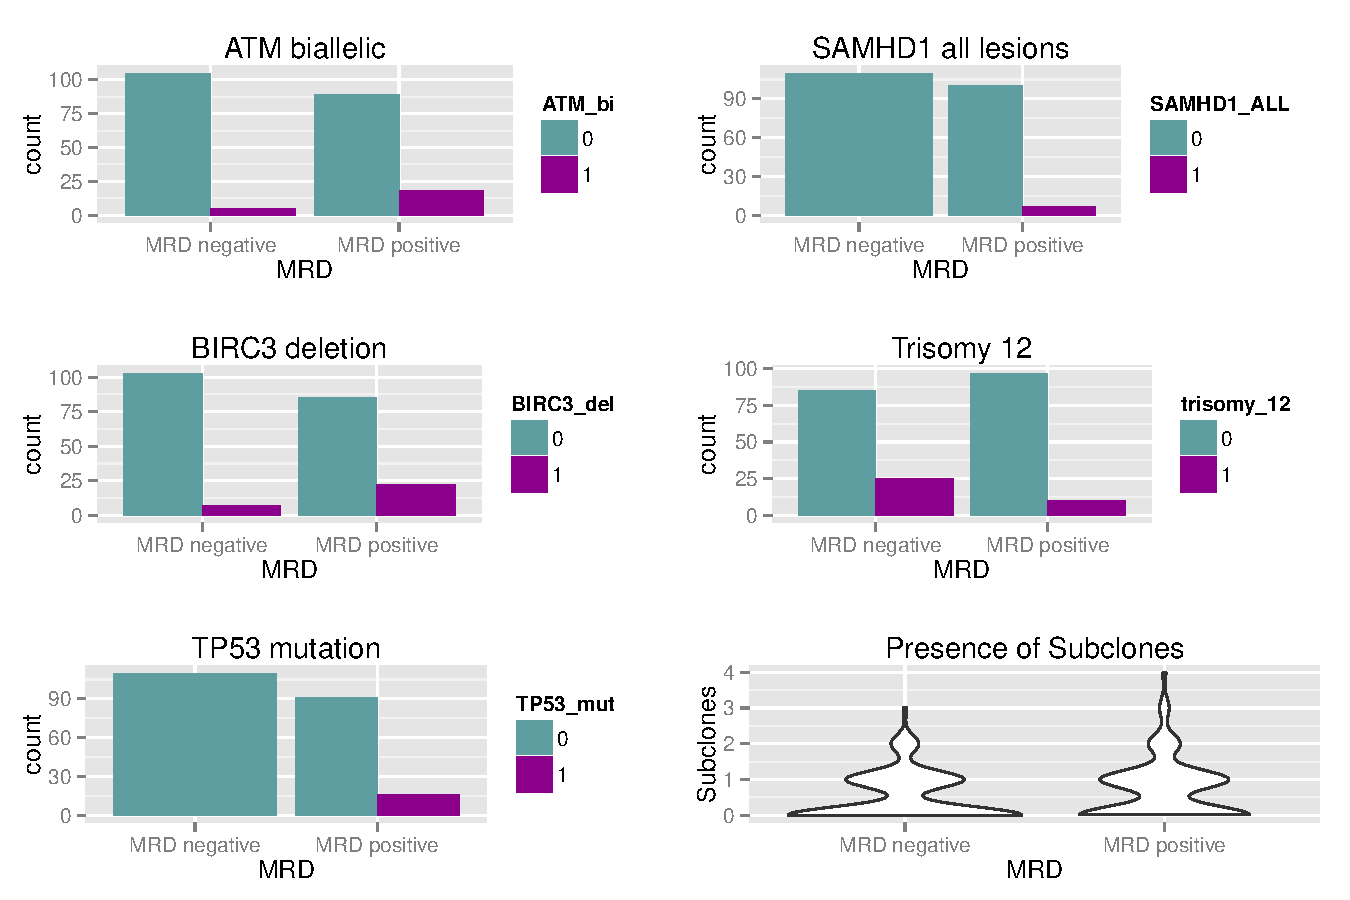
\includegraphics{HICF1_Finalreportv6-004}

\section{Associations}
To test for associations, I first counted the number of patients that have a particular mutation, and derived the probablity of having this lesion:\\
Example:\\
8 out of 217 patients have mutation X -> probability estimate for this mutation is 8/217\\
15 out of 217 patients have mutation Y ->  probability estimate for this mutation is 15/217\\
The expected probablity of having both mutations is then 8/217 x 15/217\\

I then compared this expected probability to the observed probability using Exact Binomial Tests. This test is the only one that I could find that can deal with low numbers AND allows for testing agains expected frequencies. Fisher's Exact test is often used that way by constructing the expected frequencies from the expected probabilities, but does not allow for integers, which is a problem with the low numbers we are dealing with.\\
I again used False Discovery Rate to correct the p-values.\\

\emph{This can go into a paper:}\\
We compared expected and observed probabilities using Exact Binomial Tests and corrected for mulitple testing using False Discovery Rates.


\begin{landscape}
% latex table generated in R 3.0.1 by xtable 1.7-3 package
% Tue Sep 30 08:53:02 2014
\begin{table}[ht]
\centering
{\tiny
\scalebox{0.6}{
\begin{tabular}{|r|c|c|c|c|c|c|c|c|c|c|c|c|c|c|c|c|c|c|c|c|c|c|}
  \hline
variables & TP53\_del & TP53\_cnLOH & TP53\_mut & ATM\_mut & ATM\_del & ATM\_cnLOH & BIRC3\_mut & BIRC3\_del & NOTCH1\_mut & SF3B1\_mut & X6q\_del & X13q\_ALL & trisomy\_12 & trisomy\_18 & trisomy\_19 & XPO1\_gain & SAMHD1\_ALL & MYD88mut & MED12mut & X8q\_ALL & Subclones & CNAs \\ 
  \hline
TP53\_del &  & 1.00 & 0.00 & 0.18 & 0.43 & 1.00 & 1.00 & 0.65 & 0.65 & 0.29 & 0.43 & 1.00 & 0.42 & 1.00 & 1.00 & 0.01 & 0.30 & 1.00 & 1.00 & 0.06 & 0.02 & 0.00 \\ 
  TP53\_cnLOH &  &  & 0.00 & 1.00 & 0.42 & 1.00 & 1.00 & 1.00 & 0.33 & 0.48 & 1.00 & 0.19 & 1.00 & 1.00 & 1.00 & 1.00 & 1.00 & 1.00 & 1.00 & 0.11 & 0.30 & 0.10 \\ 
  TP53\_mut &  &  &  & 0.34 & 0.20 & 1.00 & 0.65 & 0.12 & 1.00 & 1.00 & 0.33 & 0.63 & 0.09 & 1.00 & 1.00 & 0.01 & 0.53 & 1.00 & 1.00 & 0.01 & 0.00 & 0.00 \\ 
  ATM\_mut &  &  &  &  & 0.00 & 0.01 & 0.28 & 0.02 & 0.26 & 0.24 & 0.56 & 0.48 & 0.12 & 0.65 & 0.41 & 0.49 & 1.00 & 0.59 & 0.39 & 0.73 & 0.25 & 0.19 \\ 
  ATM\_del &  &  &  &  &  & 1.00 & 0.01 & 0.00 & 0.84 & 0.41 & 0.33 & 0.66 & 0.06 & 0.63 & 0.64 & 1.00 & 0.22 & 1.00 & 1.00 & 0.70 & 0.01 & 0.00 \\ 
  ATM\_cnLOH &  &  &  &  &  &  & 1.00 & 1.00 & 1.00 & 0.29 & 1.00 & 0.32 & 1.00 & 1.00 & 1.00 & 1.00 & 1.00 & 1.00 & 1.00 & 0.18 & 0.74 & 0.21 \\ 
  BIRC3\_mut &  &  &  &  &  &  &  & 0.02 & 0.06 & 1.00 & 1.00 & 0.86 & 0.04 & 0.06 & 0.01 & 1.00 & 1.00 & 1.00 & 1.00 & 0.14 & 0.90 & 0.07 \\ 
  BIRC3\_del &  &  &  &  &  &  &  &  & 0.34 & 1.00 & 0.71 & 0.80 & 0.07 & 1.00 & 1.00 & 1.00 & 0.12 & 1.00 & 1.00 & 1.00 & 0.05 & 0.06 \\ 
  NOTCH1\_mut &  &  &  &  &  &  &  &  &  & 0.13 & 1.00 & 0.12 & 0.02 & 0.55 & 0.60 & 0.38 & 1.00 & 1.00 & 0.55 & 0.38 & 0.10 & 0.84 \\ 
  SF3B1\_mut &  &  &  &  &  &  &  &  &  &  & 0.55 & 0.61 & 0.00 & 1.00 & 1.00 & 0.29 & 0.27 & 1.00 & 1.00 & 0.17 & 0.94 & 0.17 \\ 
  X6q\_del &  &  &  &  &  &  &  &  &  &  &  & 0.85 & 1.00 & 1.00 & 1.00 & 0.43 & 1.00 & 1.00 & 1.00 & 1.00 & 0.58 & 0.00 \\ 
  X13q\_ALL &  &  &  &  &  &  &  &  &  &  &  &  & 0.00 & 0.77 & 1.00 & 0.82 & 0.81 & 0.46 & 0.13 & 0.36 & 0.00 & 0.00 \\ 
  trisomy\_12 &  &  &  &  &  &  &  &  &  &  &  &  &  & 0.02 & 0.00 & 0.42 & 0.41 & 1.00 & 0.07 & 0.68 & 0.00 & 0.51 \\ 
  trisomy\_18 &  &  &  &  &  &  &  &  &  &  &  &  &  &  & 0.00 & 1.00 & 1.00 & 0.09 & 1.00 & 1.00 & 0.51 & 0.01 \\ 
  trisomy\_19 &  &  &  &  &  &  &  &  &  &  &  &  &  &  &  & 1.00 & 1.00 & 1.00 & 1.00 & 1.00 & 0.79 & 0.05 \\ 
  XPO1\_gain &  &  &  &  &  &  &  &  &  &  &  &  &  &  &  &  & 0.30 & 1.00 & 1.00 & 0.33 & 0.04 & 0.00 \\ 
  SAMHD1\_ALL &  &  &  &  &  &  &  &  &  &  &  &  &  &  &  &  &  & 1.00 & 1.00 & 1.00 & 0.68 & 0.18 \\ 
  MYD88mut &  &  &  &  &  &  &  &  &  &  &  &  &  &  &  &  &  &  & 1.00 & 1.00 & 0.65 & 0.90 \\ 
  MED12mut &  &  &  &  &  &  &  &  &  &  &  &  &  &  &  &  &  &  &  & 1.00 & 0.51 & 0.48 \\ 
  X8q\_ALL &  &  &  &  &  &  &  &  &  &  &  &  &  &  &  &  &  &  &  &  & 0.35 & 0.01 \\ 
  Subclones &  &  &  &  &  &  &  &  &  &  &  &  &  &  &  &  &  &  &  &  &  & 0.00 \\ 
  CNAs &  &  &  &  &  &  &  &  &  &  &  &  &  &  &  &  &  &  &  &  &  &  \\ 
   \hline
\end{tabular}
}
}
\caption{Association chart, uncorrected pvalues, Fisher's test} 
\end{table}
% latex table generated in R 3.0.1 by xtable 1.7-3 package
% Tue Sep 30 08:53:02 2014
\begin{table}[ht]
\centering
{\tiny
\scalebox{0.6}{
\begin{tabular}{|r|c|c|c|c|c|c|c|c|c|c|c|c|c|c|c|c|c|c|c|c|c|c|}
  \hline
variables & TP53\_del & TP53\_cnLOH & TP53\_mut & ATM\_mut & ATM\_del & ATM\_cnLOH & BIRC3\_mut & BIRC3\_del & NOTCH1\_mut & SF3B1\_mut & X6q\_del & X13q\_ALL & trisomy\_12 & trisomy\_18 & trisomy\_19 & XPO1\_gain & SAMHD1\_ALL & MYD88mut & MED12mut & X8q\_ALL & Subclones & CNAs \\ 
  \hline
TP53\_del &  & 1.00 & 0.00 & 0.69 & 1.00 & 1.00 & 1.00 & 1.00 & 1.00 & 0.91 & 1.00 & 1.00 & 1.00 & 1.00 & 1.00 & 0.09 & 0.91 & 1.00 & 1.00 & 0.35 & 0.13 & 0.00 \\ 
  TP53\_cnLOH &  &  & 0.04 & 1.00 & 1.00 & 1.00 & 1.00 & 1.00 & 0.93 & 1.00 & 1.00 & 0.70 & 1.00 & 1.00 & 1.00 & 1.00 & 1.00 & 1.00 & 1.00 & 0.53 & 0.91 & 0.49 \\ 
  TP53\_mut &  &  &  & 0.94 & 0.70 & 1.00 & 1.00 & 0.54 & 1.00 & 1.00 & 0.93 & 1.00 & 0.45 & 1.00 & 1.00 & 0.09 & 1.00 & 1.00 & 1.00 & 0.09 & 0.05 & 0.00 \\ 
  ATM\_mut &  &  &  &  & 0.05 & 0.07 & 0.90 & 0.17 & 0.88 & 0.82 & 1.00 & 1.00 & 0.54 & 1.00 & 1.00 & 1.00 & 1.00 & 1.00 & 1.00 & 1.00 & 0.84 & 0.70 \\ 
  ATM\_del &  &  &  &  &  & 1.00 & 0.09 & 0.00 & 1.00 & 1.00 & 0.93 & 1.00 & 0.34 & 1.00 & 1.00 & 1.00 & 0.78 & 1.00 & 1.00 & 1.00 & 0.09 & 0.01 \\ 
  ATM\_cnLOH &  &  &  &  &  &  & 1.00 & 1.00 & 1.00 & 0.91 & 1.00 & 0.93 & 1.00 & 1.00 & 1.00 & 1.00 & 1.00 & 1.00 & 1.00 & 0.69 & 1.00 & 0.75 \\ 
  BIRC3\_mut &  &  &  &  &  &  &  & 0.16 & 0.35 & 1.00 & 1.00 & 1.00 & 0.30 & 0.35 & 0.09 & 1.00 & 1.00 & 1.00 & 1.00 & 0.56 & 1.00 & 0.39 \\ 
  BIRC3\_del &  &  &  &  &  &  &  &  & 0.94 & 1.00 & 1.00 & 1.00 & 0.39 & 1.00 & 1.00 & 1.00 & 0.54 & 1.00 & 1.00 & 1.00 & 0.31 & 0.35 \\ 
  NOTCH1\_mut &  &  &  &  &  &  &  &  &  & 0.55 & 1.00 & 0.54 & 0.17 & 1.00 & 1.00 & 1.00 & 1.00 & 1.00 & 1.00 & 1.00 & 0.49 & 1.00 \\ 
  SF3B1\_mut &  &  &  &  &  &  &  &  &  &  & 1.00 & 1.00 & 0.04 & 1.00 & 1.00 & 0.91 & 0.90 & 1.00 & 1.00 & 0.69 & 1.00 & 0.69 \\ 
  X6q\_del &  &  &  &  &  &  &  &  &  &  &  & 1.00 & 1.00 & 1.00 & 1.00 & 1.00 & 1.00 & 1.00 & 1.00 & 1.00 & 1.00 & 0.00 \\ 
  X13q\_ALL &  &  &  &  &  &  &  &  &  &  &  &  & 0.00 & 1.00 & 1.00 & 1.00 & 1.00 & 1.00 & 0.55 & 0.96 & 0.00 & 0.00 \\ 
  trisomy\_12 &  &  &  &  &  &  &  &  &  &  &  &  &  & 0.13 & 0.02 & 1.00 & 1.00 & 1.00 & 0.39 & 1.00 & 0.06 & 1.00 \\ 
  trisomy\_18 &  &  &  &  &  &  &  &  &  &  &  &  &  &  & 0.00 & 1.00 & 1.00 & 0.46 & 1.00 & 1.00 & 1.00 & 0.09 \\ 
  trisomy\_19 &  &  &  &  &  &  &  &  &  &  &  &  &  &  &  & 1.00 & 1.00 & 1.00 & 1.00 & 1.00 & 1.00 & 0.30 \\ 
  XPO1\_gain &  &  &  &  &  &  &  &  &  &  &  &  &  &  &  &  & 0.91 & 1.00 & 1.00 & 0.93 & 0.25 & 0.01 \\ 
  SAMHD1\_ALL &  &  &  &  &  &  &  &  &  &  &  &  &  &  &  &  &  & 1.00 & 1.00 & 1.00 & 1.00 & 0.69 \\ 
  MYD88mut &  &  &  &  &  &  &  &  &  &  &  &  &  &  &  &  &  &  & 1.00 & 1.00 & 1.00 & 1.00 \\ 
  MED12mut &  &  &  &  &  &  &  &  &  &  &  &  &  &  &  &  &  &  &  & 1.00 & 1.00 & 1.00 \\ 
  X8q\_ALL &  &  &  &  &  &  &  &  &  &  &  &  &  &  &  &  &  &  &  &  & 0.95 & 0.09 \\ 
  Subclones &  &  &  &  &  &  &  &  &  &  &  &  &  &  &  &  &  &  &  &  &  & 0.00 \\ 
  CNAs &  &  &  &  &  &  &  &  &  &  &  &  &  &  &  &  &  &  &  &  &  &  \\ 
   \hline
\end{tabular}
}
}
\caption{Association chart, corrected pvalues, Fisher's test with FDR correction} 
\end{table} \end{landscape}

Odds ratios and p-values for associations between genes are represented in this heatmap. Note that odds ratios 0-1 (the first bar in the colour key) are mutually exclusive, everything else already counts as co-occuring.\\
\emph{Note: Colour key still needs be adjusted to a somewhat funny scale to see this properly.}\\
\emph{This can go into a paper:}\\
Odds ratios and significant values for associations between genes are represented in this graph. Odds ratios between 0 and 1 indicate mutually exclusive genes, while odds ratios above 1 indicate increasing co\-occurence. P-values are defined as follows: ***: p<0.001, **: p<0.01, *: p<0.05, t:trend, p<0.15
\begin{landscape}
% latex table generated in R 3.0.1 by xtable 1.7-3 package
% Tue Sep 30 08:53:03 2014
\begin{table}[ht]
\centering
{\tiny
\scalebox{0.6}{
\begin{tabular}{|r|c|c|c|c|c|c|c|c|c|c|c|c|c|c|c|c|c|c|c|c|c|c|}
  \hline
variables & TP53\_del & TP53\_cnLOH & TP53\_mut & ATM\_mut & ATM\_del & ATM\_cnLOH & BIRC3\_mut & BIRC3\_del & NOTCH1\_mut & SF3B1\_mut & X6q\_del & X13q\_ALL & trisomy\_12 & trisomy\_18 & trisomy\_19 & XPO1\_gain & SAMHD1\_ALL & MYD88mut & MED12mut & X8q\_ALL & Subclones & CNAs \\ 
  \hline
TP53\_del &  & 0.00 & 12.36 & 0.00 & 0.00 & 0.00 & 0.00 & 0.00 & 0.00 & 0.00 & 1.79 & 0.80 & 0.00 & 0.00 & 0.00 & 7.58 & 2.78 & 0.00 & 0.00 & 5.03 &  &  \\ 
  TP53\_cnLOH &  &  & 12.04 & 0.00 & 1.86 & 0.00 & 0.00 & 0.00 & 2.53 & 1.55 & 0.00 & 2.03 & 0.00 & 0.00 & 0.00 & 0.00 & 0.00 & 0.00 & 0.00 & 8.36 &  &  \\ 
  TP53\_mut &  &  &  & 0.42 & 0.26 & 0.00 & 0.00 & 0.00 & 0.72 & 0.88 & 1.71 & 1.16 & 0.00 & 0.00 & 0.00 & 4.82 & 1.32 & 0.00 & 0.00 & 4.82 &  &  \\ 
  ATM\_mut &  &  &  &  & 2.07 & 4.53 & 0.28 & 1.95 & 0.53 & 1.34 & 1.28 & 1.13 & 0.44 & 0.00 & 0.00 & 1.34 & 0.99 & 1.12 & 1.49 & 0.44 &  &  \\ 
  ATM\_del &  &  &  &  &  & 0.00 & 2.84 & 6.25 & 1.01 & 1.25 & 1.60 & 1.08 & 0.27 & 0.00 & 0.00 & 0.55 & 1.86 & 0.00 & 0.93 & 1.11 &  &  \\ 
  ATM\_cnLOH &  &  &  &  &  &  & 0.00 & 0.00 & 0.00 & 1.86 & 0.00 & 1.62 & 0.00 & 0.00 & 0.00 & 0.00 & 0.00 & 0.00 & 0.00 & 5.02 &  &  \\ 
  BIRC3\_mut &  &  &  &  &  &  &  & 2.89 & 2.40 & 0.87 & 0.00 & 1.01 & 2.38 & 5.24 & 6.77 & 0.00 & 0.00 & 0.00 & 0.00 & 3.14 &  &  \\ 
  BIRC3\_del &  &  &  &  &  &  &  &  & 0.45 & 0.98 & 1.08 & 1.04 & 0.19 & 0.00 & 0.00 & 0.76 & 2.54 & 0.00 & 0.00 & 0.76 &  &  \\ 
  NOTCH1\_mut &  &  &  &  &  &  &  &  &  & 0.41 & 0.54 & 0.59 & 2.13 & 1.26 & 1.08 & 1.52 & 0.84 & 0.00 & 1.26 & 1.52 &  &  \\ 
  SF3B1\_mut &  &  &  &  &  &  &  &  &  &  & 1.33 & 1.09 & 0.11 & 0.77 & 0.66 & 0.00 & 0.00 & 0.00 & 0.77 & 1.87 &  &  \\ 
  X6q\_del &  &  &  &  &  &  &  &  &  &  &  & 1.01 & 0.89 & 0.00 & 0.00 & 1.79 & 0.00 & 0.00 & 0.00 & 0.00 &  &  \\ 
  X13q\_ALL &  &  &  &  &  &  &  &  &  &  &  &  & 0.24 & 1.01 & 0.86 & 1.01 & 1.12 & 1.52 & 0.00 & 1.42 &  &  \\ 
  trisomy\_12 &  &  &  &  &  &  &  &  &  &  &  &  &  & 4.22 & 5.46 & 0.00 & 0.00 & 0.00 & 3.15 & 1.25 &  &  \\ 
  trisomy\_18 &  &  &  &  &  &  &  &  &  &  &  &  &  &  & 30.35 & 0.00 & 0.00 & 10.45 & 0.00 & 0.00 &  &  \\ 
  trisomy\_19 &  &  &  &  &  &  &  &  &  &  &  &  &  &  &  & 0.00 & 0.00 & 0.00 & 0.00 & 0.00 &  &  \\ 
  XPO1\_gain &  &  &  &  &  &  &  &  &  &  &  &  &  &  &  &  & 2.78 & 0.00 & 0.00 & 2.51 &  &  \\ 
  SAMHD1\_ALL &  &  &  &  &  &  &  &  &  &  &  &  &  &  &  &  &  & 0.00 & 0.00 & 0.00 &  &  \\ 
  MYD88mut &  &  &  &  &  &  &  &  &  &  &  &  &  &  &  &  &  &  & 0.00 & 0.00 &  &  \\ 
  MED12mut &  &  &  &  &  &  &  &  &  &  &  &  &  &  &  &  &  &  &  & 0.00 &  &  \\ 
  X8q\_ALL &  &  &  &  &  &  &  &  &  &  &  &  &  &  &  &  &  &  &  &  &  &  \\ 
  Subclones &  &  &  &  &  &  &  &  &  &  &  &  &  &  &  &  &  &  &  &  &  &  \\ 
  CNAs &  &  &  &  &  &  &  &  &  &  &  &  &  &  &  &  &  &  &  &  &  &  \\ 
   \hline
\end{tabular}
}
}
\caption{Odds ratios for association between genes} 
\end{table}\end{landscape}
\newpage

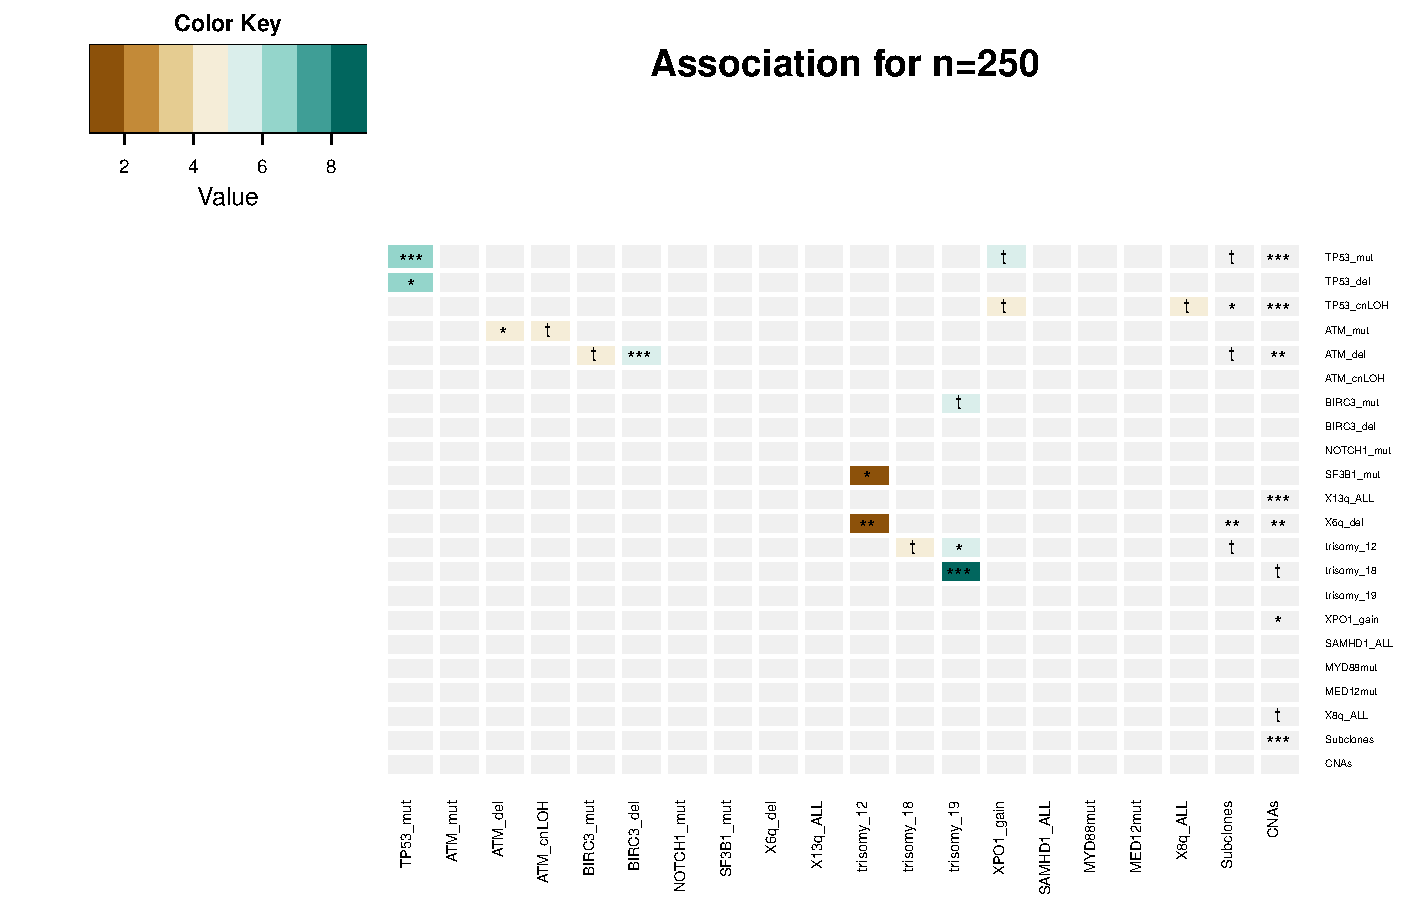
\includegraphics{HICF1_Finalreportv6-010}

\subsection{Multiple logistic regression models}

\emph{This can go into a paper:}\\
As significantly more MRD positive patients have progressed during the trial (Chi Square test, ChiSquare=10.26, n=104, p=0.001), we use MRD status as proxy for progression free survival.\\
Mulitvariate analysis was done using multiple logistic regression models. We selected only variables that were significant in the univariate analysis to go into the multiple logistic regression. One specific goal was to see if ATM biallelic is a better predictor for MRD positivity than ATM deletions.



% Table created by stargazer v.5.1 by Marek Hlavac, Harvard University. E-mail: hlavac at fas.harvard.edu
% Date and time: Tue, Sep 30, 2014 - 08:53:04
\begin{table}[!htbp] \centering 
  \caption{Multiple log regression, n=217} 
  \label{} 
\tiny 
\begin{tabular}{@{\extracolsep{5pt}}lccccccc} 
\\[-1.8ex]\hline 
\hline \\[-1.8ex] 
 & \multicolumn{7}{c}{\textit{Dependent variable:}} \\ 
\cline{2-8} 
\\[-1.8ex] & \multicolumn{7}{c}{MRD} \\ 
 & genetic1 & genetic2 & genetic3 & genetic4 & genetic5 & genetic6 & genetic7 \\ 
\hline \\[-1.8ex] 
 TP53\_ALL1 & 2.65$^{***}$ (0.77) & 2.59$^{***}$ (0.76) & 2.56$^{***}$ (0.76) & 2.56$^{***}$ (0.76) & 2.46$^{***}$ (0.76) & 2.46$^{***}$ (0.76) &  \\ 
  ATM\_del1 & 1.40$^{***}$ (0.41) &  &  &  &  &  &  \\ 
  ATM\_bi1 &  & 1.51$^{***}$ (0.54) & 1.55$^{***}$ (0.55) & 1.59$^{***}$ (0.55) & 1.55$^{***}$ (0.55) &  &  \\ 
  trisomy\_121 & $-$0.66 (0.42) & $-$0.66 (0.42) & $-$0.45 (0.43) & $-$0.52 (0.43) & $-$0.61 (0.43) &  &  \\ 
  BIRC3\_mono1 &  &  & $-$0.96 (1.33) & $-$1.70 (1.15) & $-$1.74 (1.15) &  &  \\ 
  SAMHD1\_ALL1 & 16.64 (854.98) & 16.71 (873.55) & 17.69 (1,438.54) & 16.69 (872.11) &  &  &  \\ 
  trisomy\_121:BIRC3\_mono1 &  &  & $-$15.83 (1,769.26) &  &  &  &  \\ 
  vh\_mutation\_statusunmutated &  &  &  &  &  &  & 0.16 (0.50) \\ 
  Constant & $-$0.44$^{**}$ (0.18) & $-$0.34$^{*}$ (0.17) & $-$0.32$^{*}$ (0.18) & $-$0.32$^{*}$ (0.18) & $-$0.22 (0.17) & $-$0.20 (0.14) & $-$0.22 (0.47) \\ 
 \hline \\[-1.8ex] 
Observations & 217 & 217 & 217 & 217 & 217 & 217 & 196 \\ 
Log Likelihood & $-$127.05 & $-$128.86 & $-$126.86 & $-$127.39 & $-$132.64 & $-$141.44 & $-$135.64 \\ 
Akaike Inf. Crit. & 264.11 & 267.72 & 267.71 & 266.79 & 275.29 & 286.88 & 275.29 \\ 
\hline 
\hline \\[-1.8ex] 
\textit{Note:}  & \multicolumn{7}{l}{$^{*}$p$<$0.1; $^{**}$p$<$0.05; $^{***}$p$<$0.01} \\ 
\end{tabular} 
\end{table}  
\newpage
\subsection{Missclassification Error}

% Table created by stargazer v.5.1 by Marek Hlavac, Harvard University. E-mail: hlavac at fas.harvard.edu
% Date and time: Tue, Sep 30, 2014 - 08:53:04
\begin{table}[!htbp] \centering 
  \caption{Missclassification for summarized models} 
  \label{} 
\tiny 
\begin{tabular}{@{\extracolsep{1p}} cccccccc} 
\\[-1.8ex]\hline 
\hline \\[-1.8ex] 
 & model & correct\_MRD\_neg & false\_MRD\_neg & correct\_MRD\_pos & false\_MRD\_pos & missclasserr & unclassified \\ 
\hline \\[-1.8ex] 
1 & fit.sum.gen1 & $98$ & $56$ & $51$ & $12$ & $0.313$ & $0$ \\ 
2 & fit.sum.gen2 & $103$ & $65$ & $42$ & $7$ & $0.332$ & $0$ \\ 
3 & fit.sum.gen3 & $103$ & $65$ & $42$ & $7$ & $0.332$ & $0$ \\ 
4 & fit.sum.gen4 & $103$ & $66$ & $41$ & $7$ & $0.336$ & $0$ \\ 
5 & fit.sum.gen5 & $103$ & $72$ & $35$ & $7$ & $0.364$ & $0$ \\ 
6 & fit.sum.gen6 & $108$ & $88$ & $19$ & $2$ & $0.415$ & $0$ \\ 
7 & fit.vhmut & $102$ & $94$ & $$ & $$ & $$ & $0.097$ \\ 
\hline \\[-1.8ex] 
\end{tabular} 
\end{table} \subsubsection{Model probabilities}

The following graphs show the predicted probability for MRD positivity of the different models, with the x-axis showing the real MRD status. Note again that the final model only contains 181 data points.\\
The graph depicts the following variables (note:Not all of them are necessarily in the model depicted):\\
\begin{itemize}
  \item Trisomy12 is depicted by the shape of the points (cirle=0, square=1).
  \item SAMHD1 is depicted by translucent points (translucent=mutated)
  \item ATM biallelic is depicted by light blue filling.
  \item BIRC3 is depicted by green(0) and red(1) point outline.
  \item TP53 is depicted by point size (large=1)
\end{itemize}
The dashed red line shows the 0.5 line. Everything above is classified by the model as MRD positive, below is classified as MRD negative.
\newpage

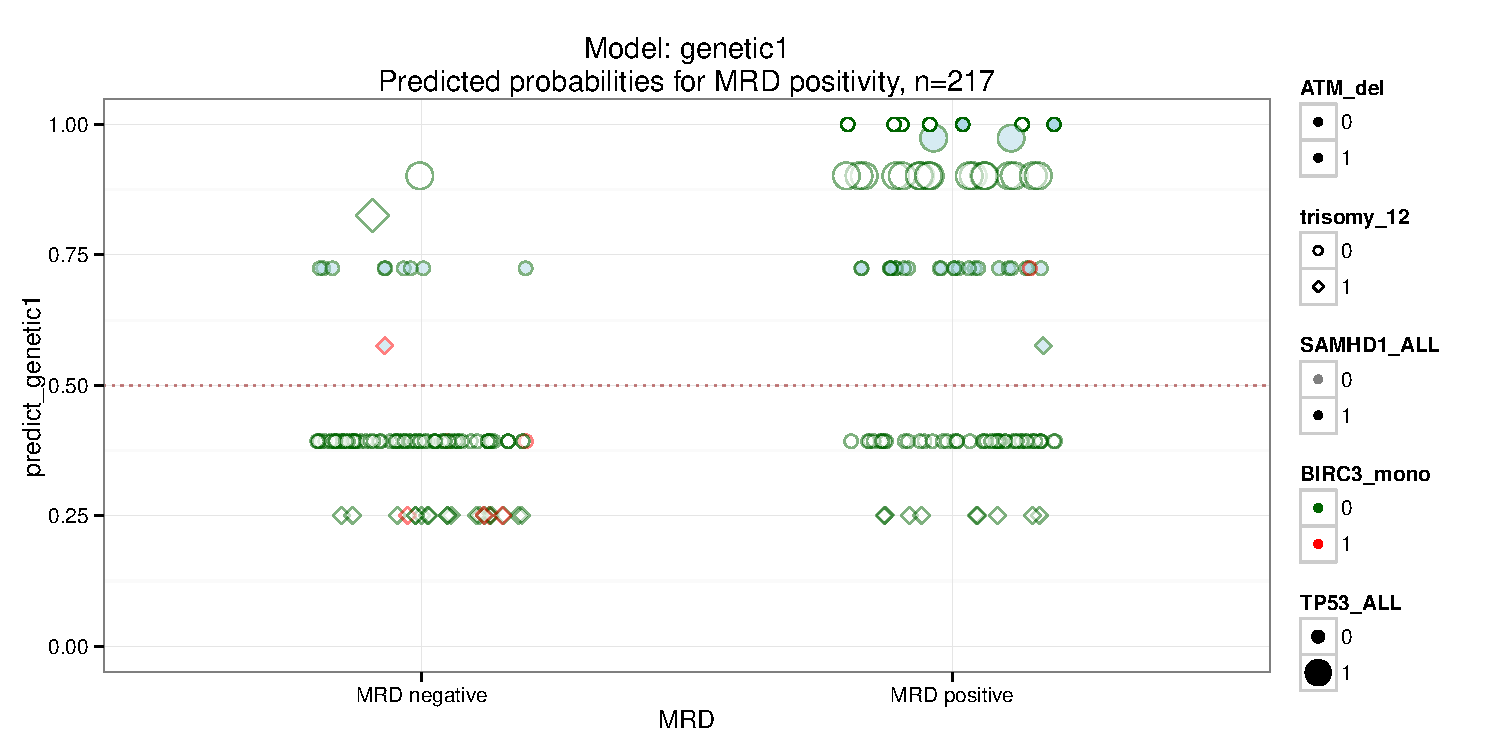
\includegraphics{HICF1_Finalreportv6-genetic1}

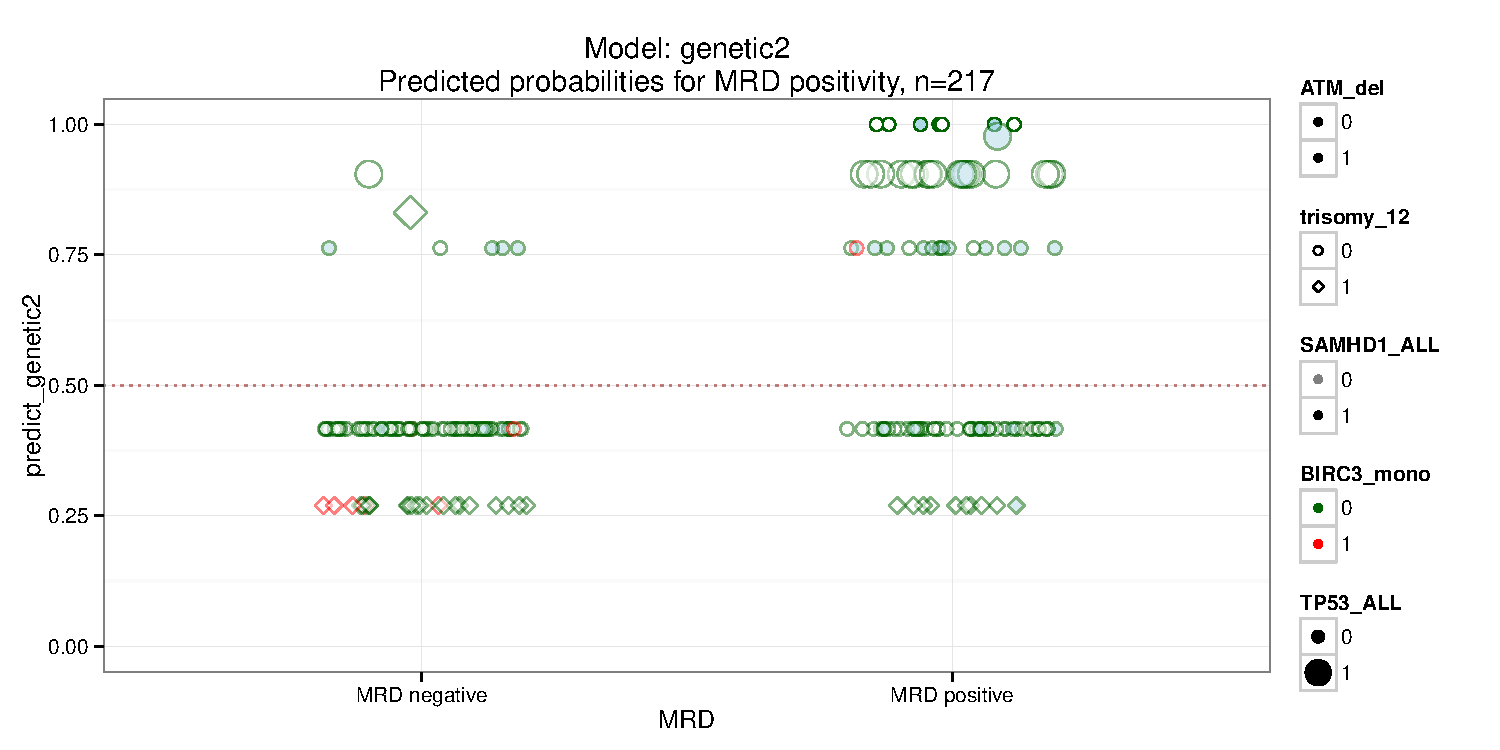
\includegraphics{HICF1_Finalreportv6-genetic2}

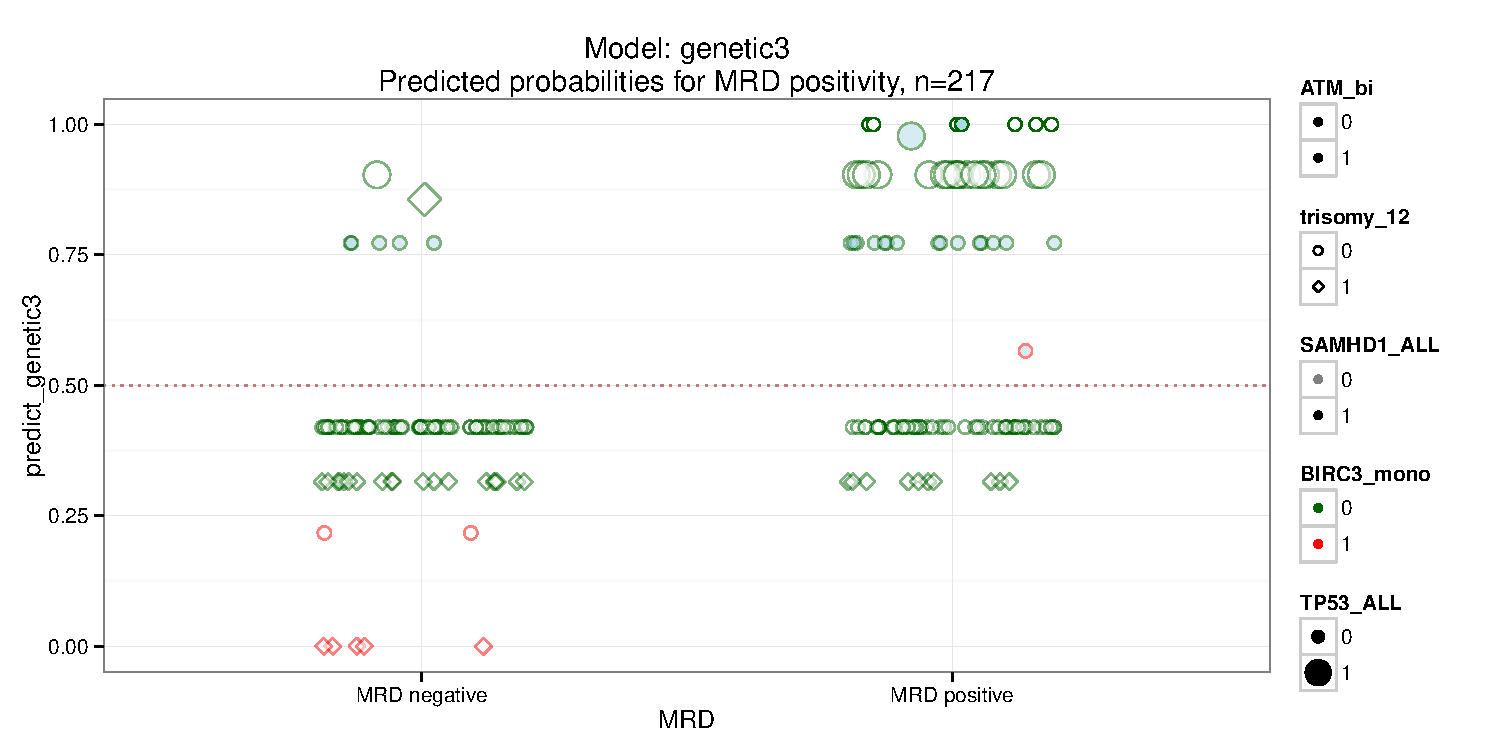
\includegraphics{HICF1_Finalreportv6-genetic3}

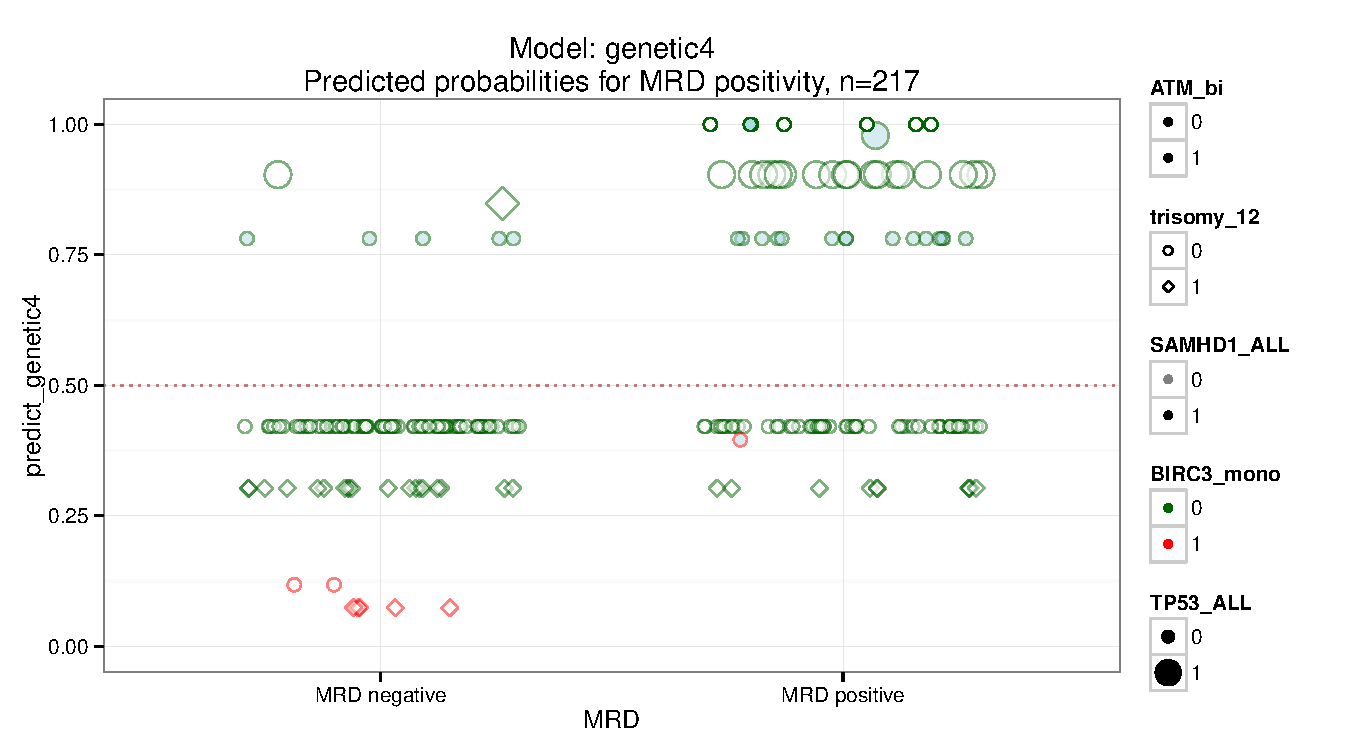
\includegraphics{HICF1_Finalreportv6-genetic4}

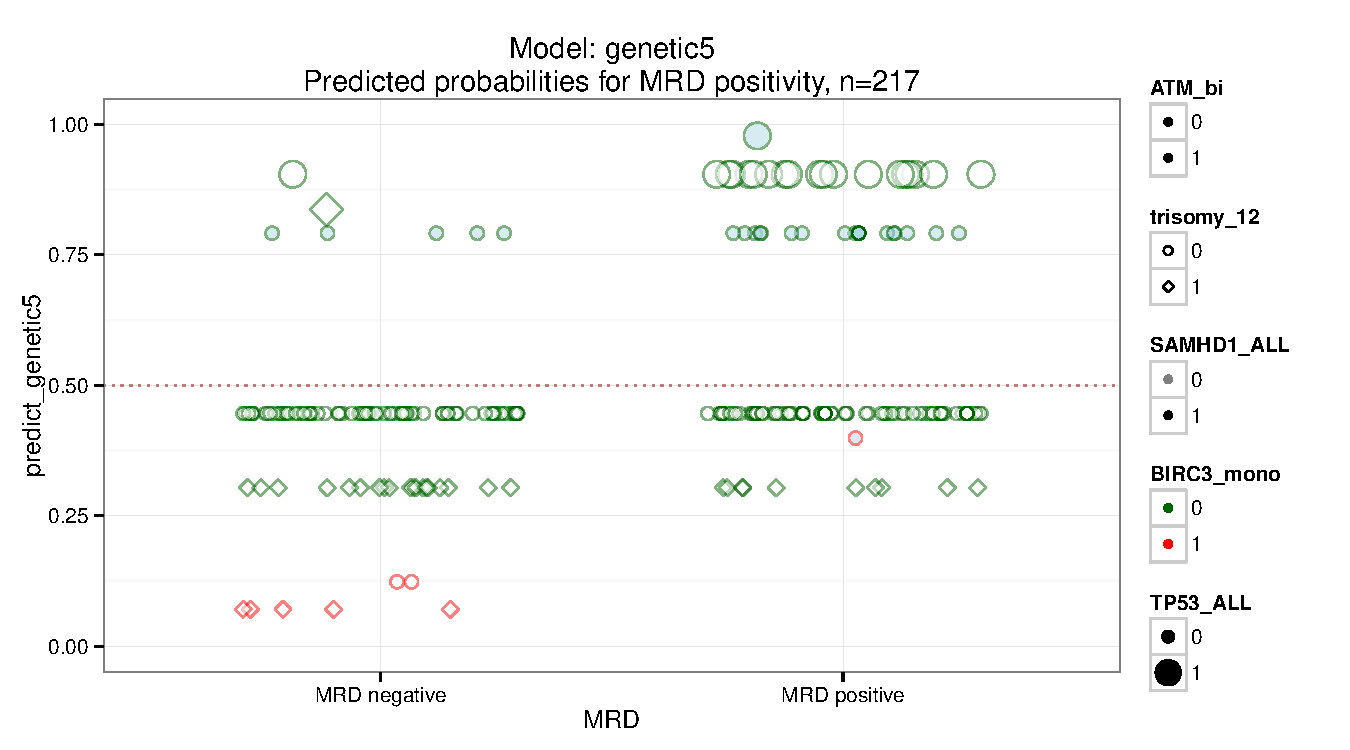
\includegraphics{HICF1_Finalreportv6-genetic5}

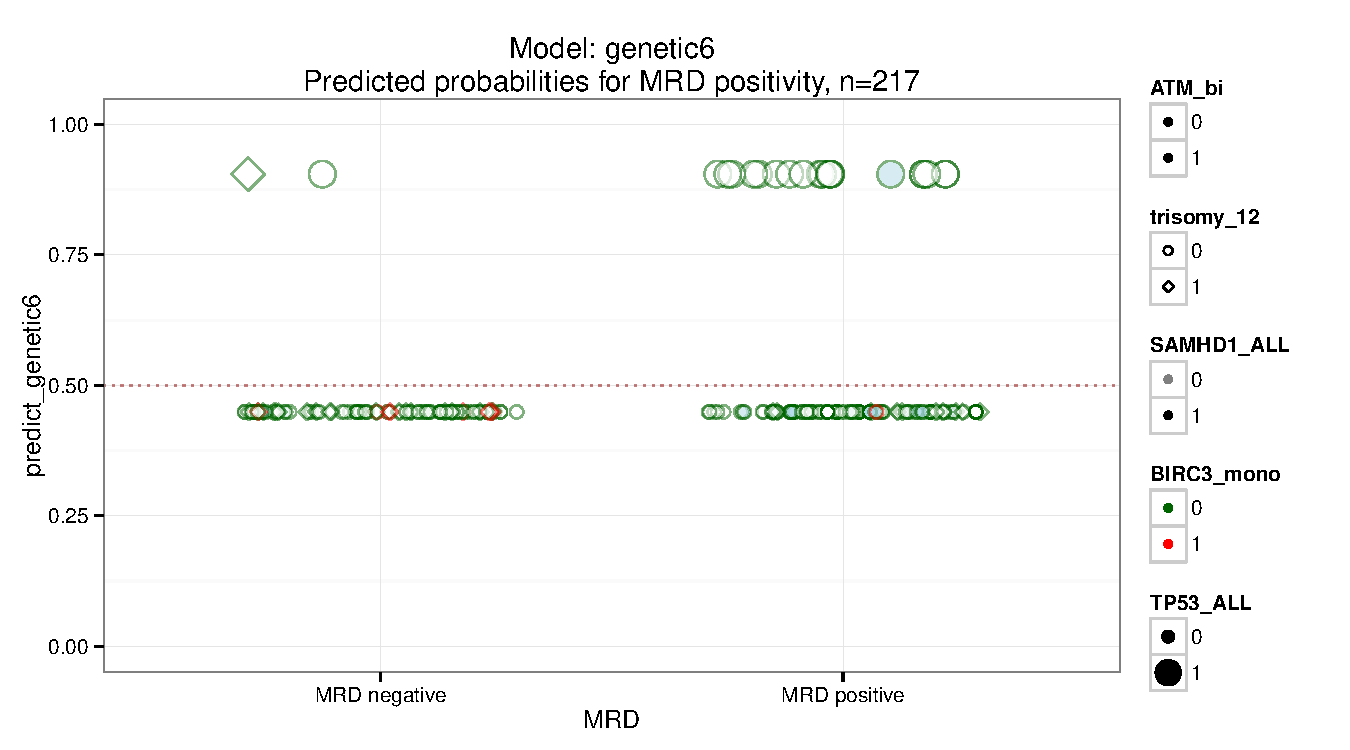
\includegraphics{HICF1_Finalreportv6-genetic6}

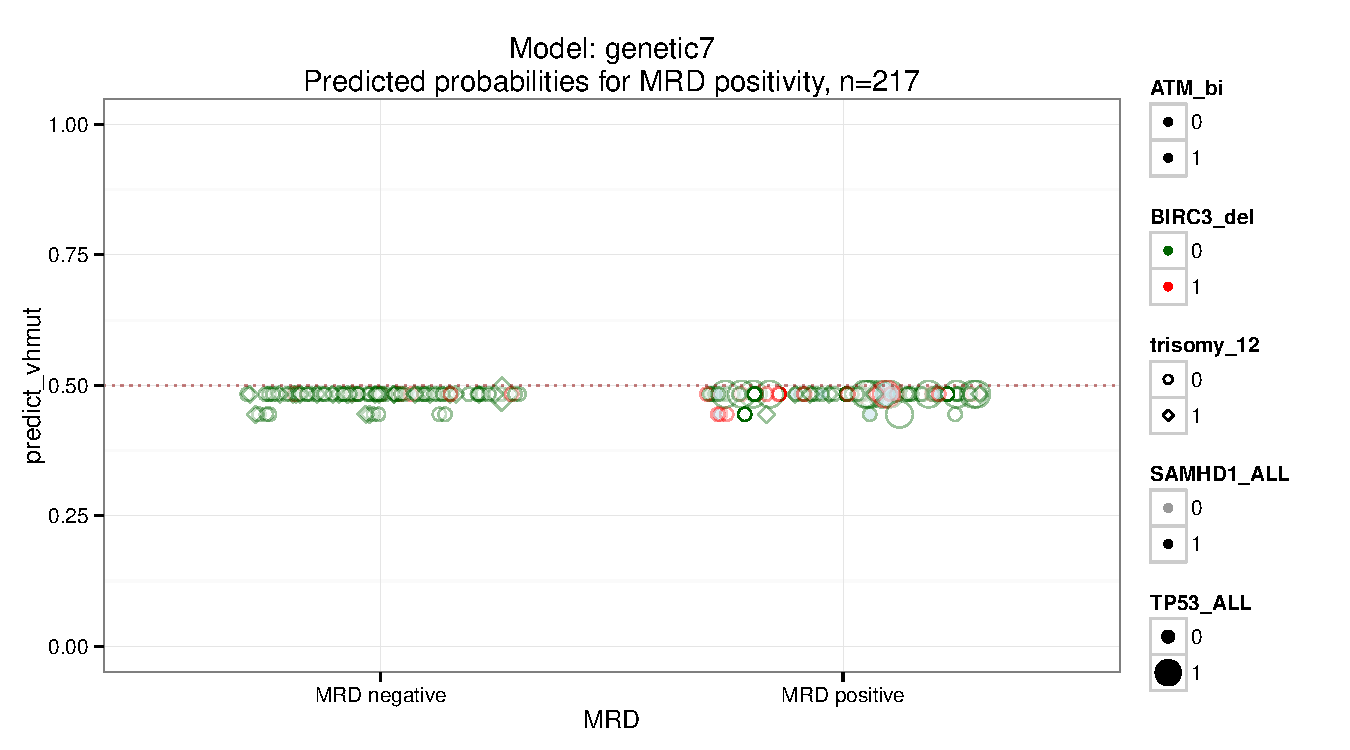
\includegraphics{HICF1_Finalreportv6-vhmut}
\subsection{Model Accuracy}
To estimate model accuracy, we selected all patients that were correctly classified and looked at their model probablities. You can see nicely that model 1, despite being the model with the best missclassification errors, is not as accurate as model 2 and 4 (both using ATM bi) for MRD positivity. \\
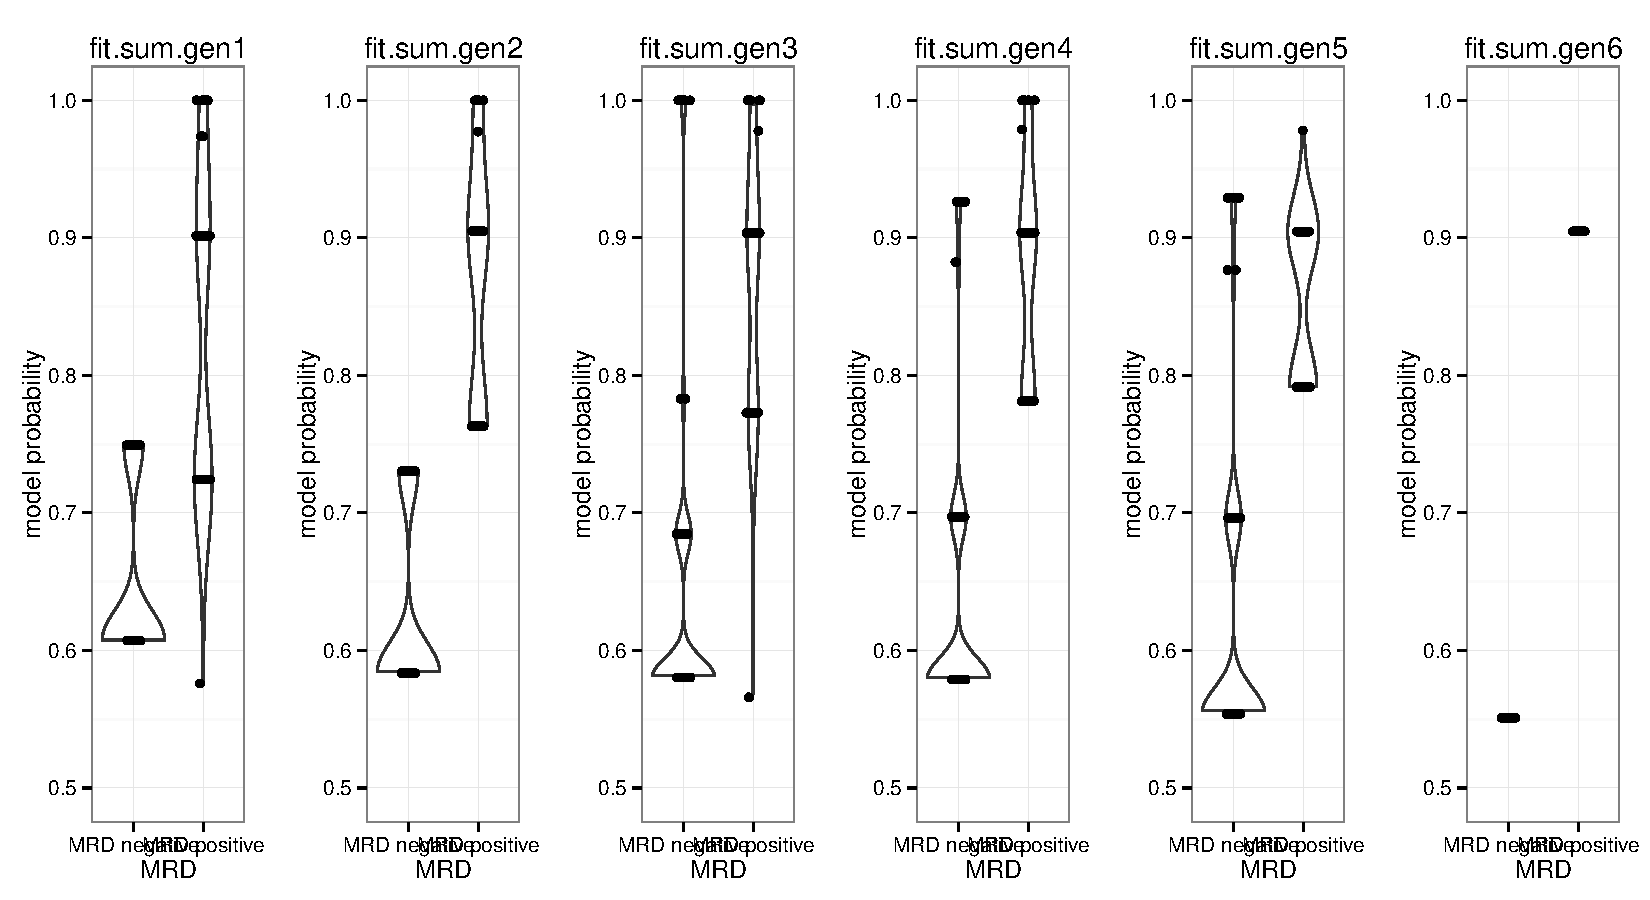
\includegraphics{HICF1_Finalreportv6-022}


% Table created by stargazer v.5.1 by Marek Hlavac, Harvard University. E-mail: hlavac at fas.harvard.edu
% Date and time: Tue, Sep 30, 2014 - 08:53:08
\begin{table}[!htbp] \centering 
  \caption{Summary model probabilities} 
  \label{} 
\small 
\begin{tabular}{@{\extracolsep{1p}} cccccccccc} 
\\[-1.8ex]\hline 
\hline \\[-1.8ex] 
 & model & +mean & +median & +min & +max & -mean & -median & -min & -max \\ 
\hline \\[-1.8ex] 
1 & fit.sum.gen1 & 83\% & 90\% & 58\% & 100\% & 64\% & 61\% & 61\% & 75\% \\ 
2 & fit.sum.gen2 & 87\% & 90\% & 76\% & 100\% & 62\% & 58\% & 58\% & 73\% \\ 
3 & fit.sum.gen3 & 87\% & 90\% & 57\% & 100\% & 62\% & 58\% & 58\% & 100\% \\ 
4 & fit.sum.gen4 & 88\% & 90\% & 78\% & 100\% & 62\% & 58\% & 58\% & 93\% \\ 
5 & fit.sum.gen5 & 85\% & 90\% & 79\% & 98\% & 60\% & 55\% & 55\% & 93\% \\ 
6 & fit.sum.gen6 & 90\% & 90\% & 90\% & 90\% & 55\% & 55\% & 55\% & 55\% \\ 
\hline \\[-1.8ex] 
\end{tabular} 
\end{table} 
% You can see that using only vh mutation status leads to a somewhat cloudy prediction with quite a lot of false positives. The genetic model (on the very top) as well as the combination of vh mutation status and genetic features lead to a more distinctive distribution, and fewer false positives.
% 
% \subsubsection{Generalization through machine learning}
% Next we want to know how our model performs when applied more generally. In order to do that, we devide the data into a training data and a test data set an assess its performance.
% As we do not have a validation data set, we will use a method called cross-validation (CV): We repeatedly (1000 times) choose a random subset of our data (about 10\%) to be left out and serve as a validation set, then calculate the error and variation from this.
% \newpage
% 
% <<ML model performance, echo=FALSE, eval=TRUE>>=
% source("/home/andreas/suska/work/01_HICF1/HICF1_sub1/trunk/HICF1_v7/cv_logreg.R")
% #make dataframe only with target columns
% #GENETIC MODEL
% genetic3_variables <- c("TP53_ALL", "ATM_bi", "Trisomy_12", "SAMHD1_ALL", "MRD")
% genclinv6_genetic3 <- model.genclinv6[,colnames(model.genclinv6) %in% genetic3_variables]
% rownames(genclinv6_genetic3) <- NULL
% performance_genetic3 <- cv_logreg(genclinv6_genetic3)
% @
% 
% <<fig=TRUE, echo=FALSE, width=7, height=4>>=
% require(reshape2)
% performance_genetic3.sum <- melt(performance_genetic3, id.vars=c("model.no"))
% performance_genetic3.sum$variable <- as.factor(performance_genetic3.sum$variable)
% 
% ggplot(performance_genetic3.sum, aes(x=variable, y=value))+
%   geom_boxplot(colour=c("firebrick4", "green",  "darkolivegreen", "firebrick1","darkgrey"), outlier.shape = NA)+
%   geom_point(position = position_jitter(w = 0.1), alpha=0.02)+
%   ylab("Fraction of total no of patients in test set")+
%   ggtitle("Repeated random sub-sampling for genetic data in log regression model,\nnrepeat=1000")+
%   ylim(c(0, 1))
% @
% 
% <<ML model performance, echo=FALSE, eval=TRUE>>=
% source("/home/andreas/suska/work/01_HICF1/HICF1_sub1/trunk/HICF1_v7/cv_logreg.R")
% #make dataframe only with target columns
% #VHMUT MODEL
% vhmut_variables <- c("vh_mutation_status", "MRD")
% vhmut_performancedata <- model.genclinv6.vhmut[,colnames(model.genclinv6.vhmut) %in% vhmut_variables]
% rownames(vhmut_performancedata) <- NULL
% performance_vhmut <- cv_logreg(vhmut_performancedata)
% @
% 
% <<fig=TRUE, echo=FALSE, width=7, height=4>>=
% require(reshape2)
% performance_vhmut.sum <- melt(performance_vhmut, id.vars=c("model.no"))
% performance_vhmut.sum$variable <- as.factor(performance_vhmut.sum$variable)
% 
% ggplot(performance_vhmut.sum, aes(x=variable, y=value))+
%   geom_boxplot(colour=c("firebrick4", "green",  "darkolivegreen", "firebrick1","darkgrey"),outlier.shape = NA)+
%   geom_point(position = position_jitter(w = 0.1), alpha=0.02)+
%   ylab("Fraction of total no of patients in test set")+
%   ggtitle("Repeated random sub-sampling for vhmut data in log regression model,\nnrepeat=1000")+
%   ylim(c(0, 1))
% @
% 
% <<ML model performance, echo=FALSE, eval=TRUE>>=
% source("/home/andreas/suska/work/01_HICF1/HICF1_sub1/trunk/HICF1_v7/cv_logreg.R")
% #make dataframe only with target columns
% #VHMUT+GENETIC MODEL
% vhmutgenetic_variables <- c("TP53_ALL", "ATM_bi", "Trisomy_12", "SAMHD1_ALL","vh_mutation_status", "MRD")
% vhmutgenetic_performancedata <- model.genclinv6.vhmut[,colnames(model.genclinv6.vhmut) %in% vhmutgenetic_variables]
% rownames(vhmutgenetic_performancedata) <- NULL
% performance_vhmutgenetic <- cv_logreg(vhmutgenetic_performancedata)
% @
% 
% <<fig=TRUE, echo=FALSE, width=7, height=4>>=
% require(reshape2)
% performance_vhmutgenetic.sum <- melt(performance_vhmutgenetic, id.vars=c("model.no"))
% performance_vhmutgenetic.sum$variable <- as.factor(performance_vhmutgenetic.sum$variable)
% 
% ggplot(performance_vhmutgenetic.sum, aes(x=variable, y=value))+
%   geom_boxplot(colour=c("firebrick4", "green",  "darkolivegreen", "firebrick1","darkgrey"),outlier.shape = NA)+
%   geom_point(position = position_jitter(w = 0.1), alpha=0.02)+
%   ylab("Fraction of total no of patients in test set")+
%   ggtitle("Repeated random sub-sampling for vhmutgenetic data in log regression model,\nnrepeat=1000")+
%   ylim(c(0, 1))
% @
% \newpage
% This is basically the same data displayed for all three models in one graph for better comparison. You can see that the genetic model performs similar to the vh mutation, with the ADVANTAGE of classifying all the patients,It is also slightly more reliable in picking up true MRD positives (truenegative) and MRD negatives (truepositives). All three models have quite some error(ranging beyond the 50\% mark, which is guessing), so the take home message here should be: The genetic testing performs AS GOOD AS vh mutation status, but includes all patients.
% 
% <<fig=TRUE, echo=FALSE, width=9, height=6>>=
% library(reshape2)
% library(plyr)
% combined_models <- ldply(list(genetic3=performance_genetic3.sum, vhmut = performance_vhmut.sum, geneticvhmut=performance_vhmutgenetic.sum))
% ggplot(combined_models, aes(variable, value, dodge = .id, colour=.id)) +
%   geom_boxplot(position = position_dodge(width = 0.8),outlier.shape = NA)+
%   ggtitle("Comparison of model performance")
% @
% \newpage

\section{Progression Free Survival}

\subsection{MRD as Proxy for PFS}
We first assess if MRD is a good proxy for survival via simple univariate testing:\\
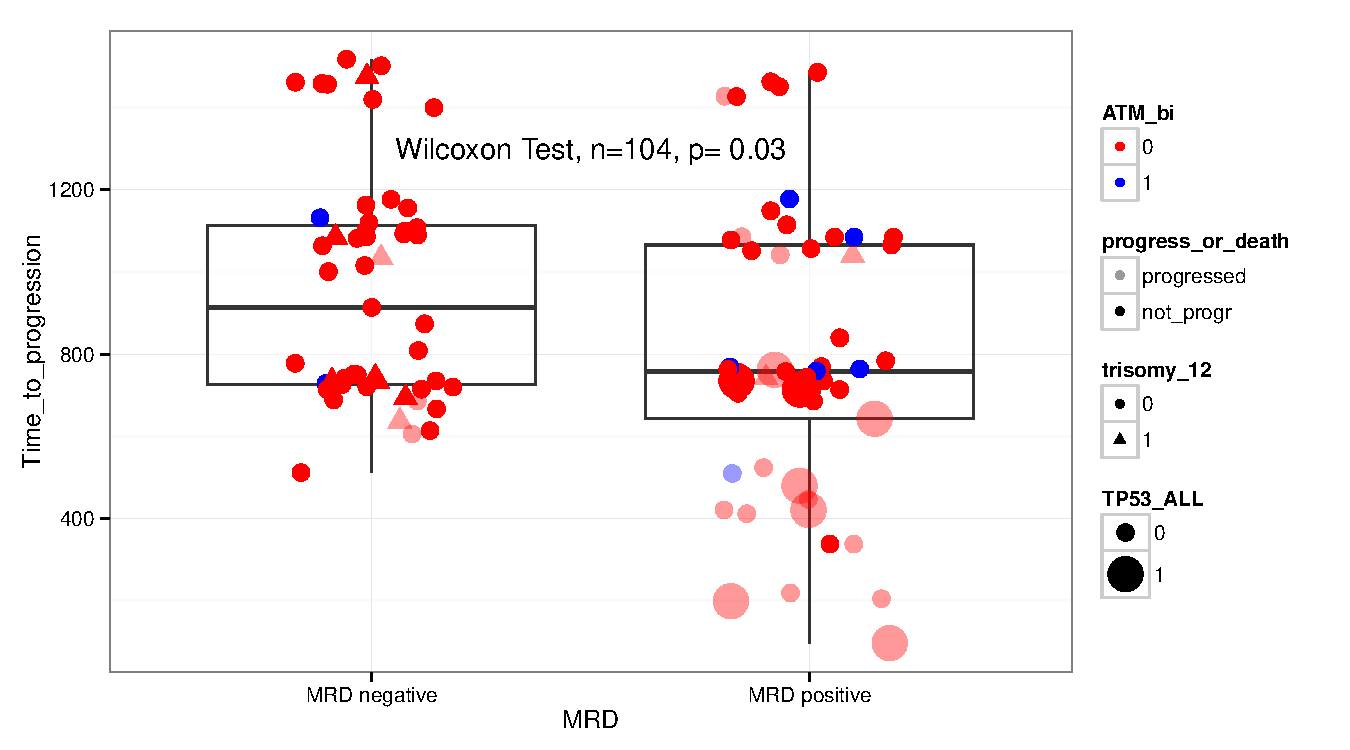
\includegraphics{HICF1_Finalreportv6-025}


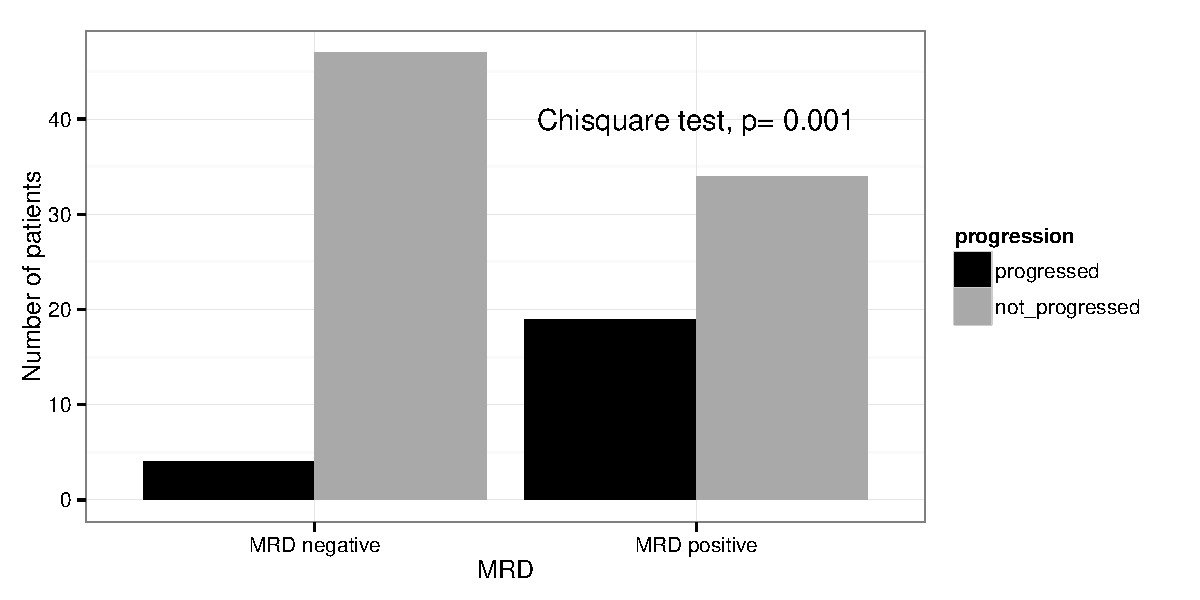
\includegraphics{HICF1_Finalreportv6-027}

\\ We can conclude that MRD is a good proxy for PFS.\\
Next, we want to check if progression is biased towards a certain gender or age:\\
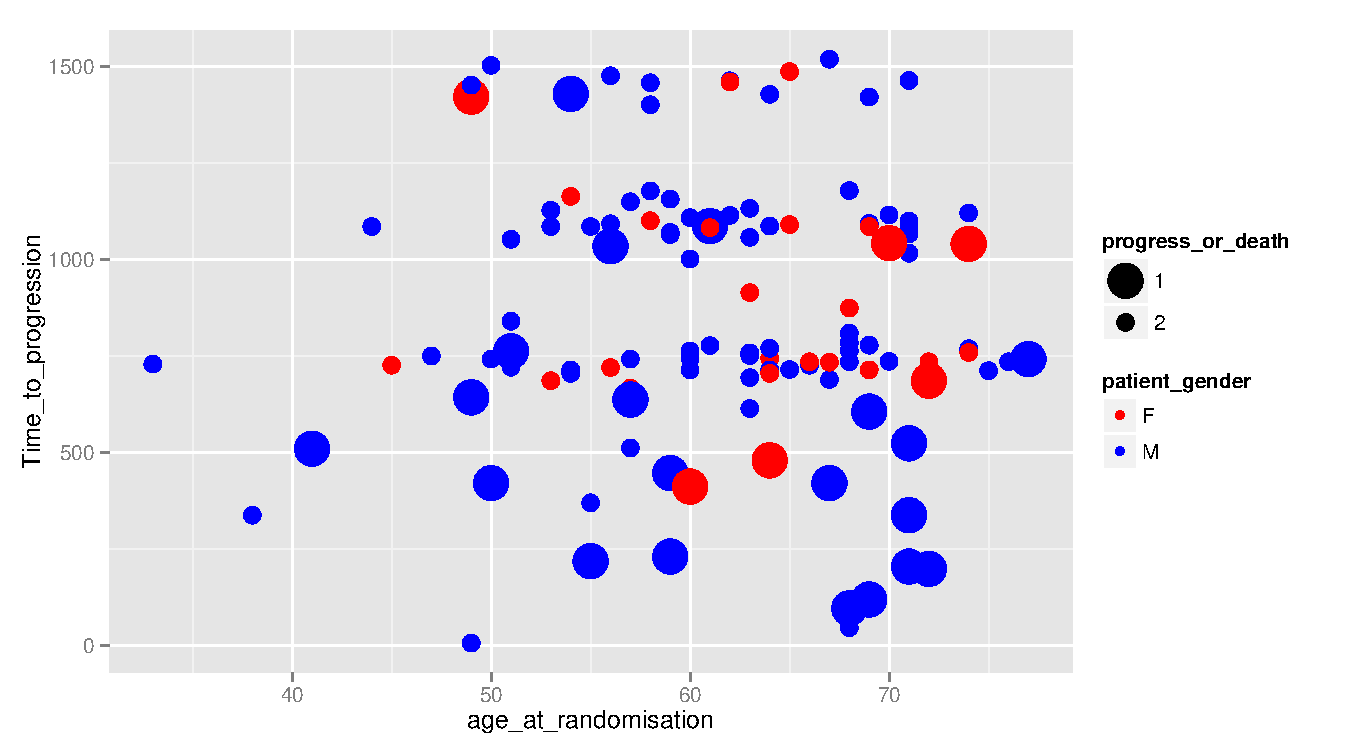
\includegraphics{HICF1_Finalreportv6-028}
\\Fortunately, this is not the case, although we have double thenumber of males compared to females, both age and gender does not confound with pregression and time to progression.
\subsection{Cox Hazard Regression Model}
First, we plot all our data to see how it looks like in a Kaplan-Meier Curve:\\

% Table created by stargazer v.5.1 by Marek Hlavac, Harvard University. E-mail: hlavac at fas.harvard.edu
% Date and time: Tue, Sep 30, 2014 - 08:53:09
\begin{table}[!htbp] \centering 
  \caption{Survival model} 
  \label{} 
\small 
\begin{tabular}{@{\extracolsep{5pt}}lc} 
\\[-1.8ex]\hline 
\hline \\[-1.8ex] 
 & \multicolumn{1}{c}{\textit{Dependent variable:}} \\ 
\cline{2-2} 
\\[-1.8ex] & Time\_to\_progression \\ 
\hline \\[-1.8ex] 
 TP53\_ALL1 & 2.38$^{***}$ (0.51) \\ 
  ATM\_bi1 & 0.19 (1.06) \\ 
  SAMHD1\_ALL1 & 2.82$^{***}$ (0.61) \\ 
  trisomy\_121 & 1.08$^{*}$ (0.59) \\ 
 \hline \\[-1.8ex] 
Observations & 118 \\ 
R$^{2}$ & 0.21 \\ 
Max. Possible R$^{2}$ & 0.85 \\ 
Log Likelihood & $-$98.03 \\ 
Wald Test & 32.56$^{***}$ (df = 4) \\ 
LR Test & 27.90$^{***}$ (df = 4) \\ 
Score (Logrank) Test & 50.83$^{***}$ (df = 4) \\ 
\hline 
\hline \\[-1.8ex] 
\textit{Note:}  & \multicolumn{1}{l}{$^{*}$p$<$0.1; $^{**}$p$<$0.05; $^{***}$p$<$0.01} \\ 
\end{tabular} 
\end{table} 
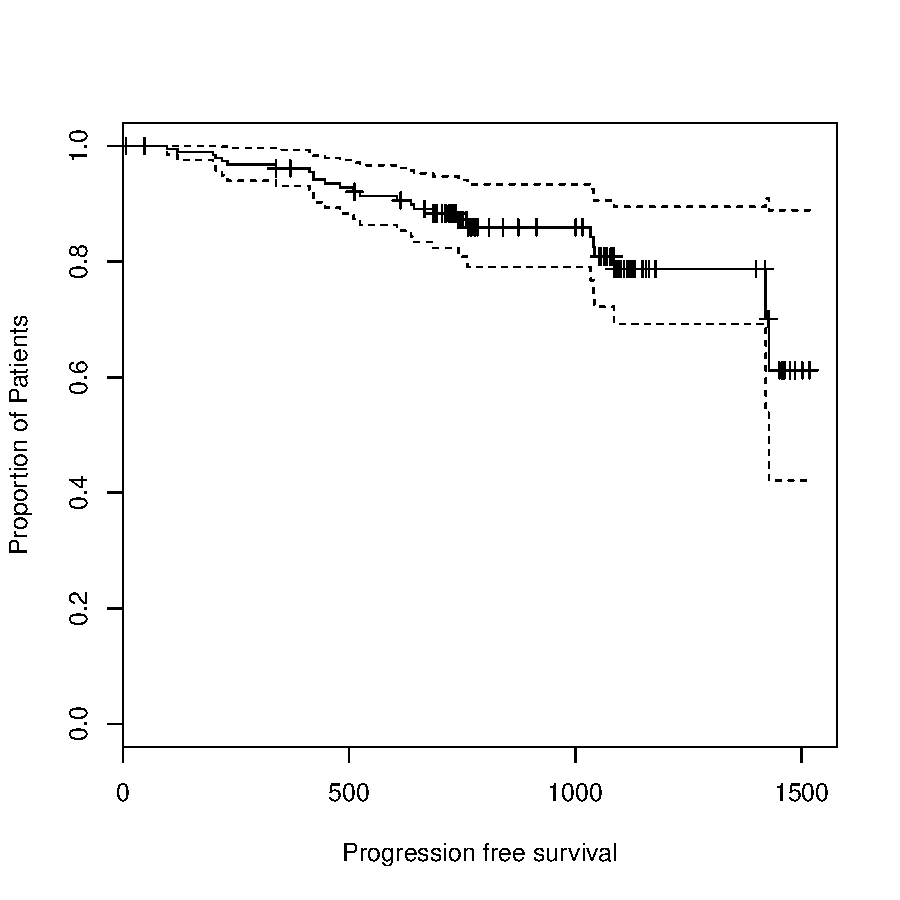
\includegraphics{HICF1_Finalreportv6-031}
\\We fitted a Cox Proportional Hazard Model using the survival package (R), with TP53, ATM biallelic, SAMHD1 and trisomy 12 as predictors.\\
\\
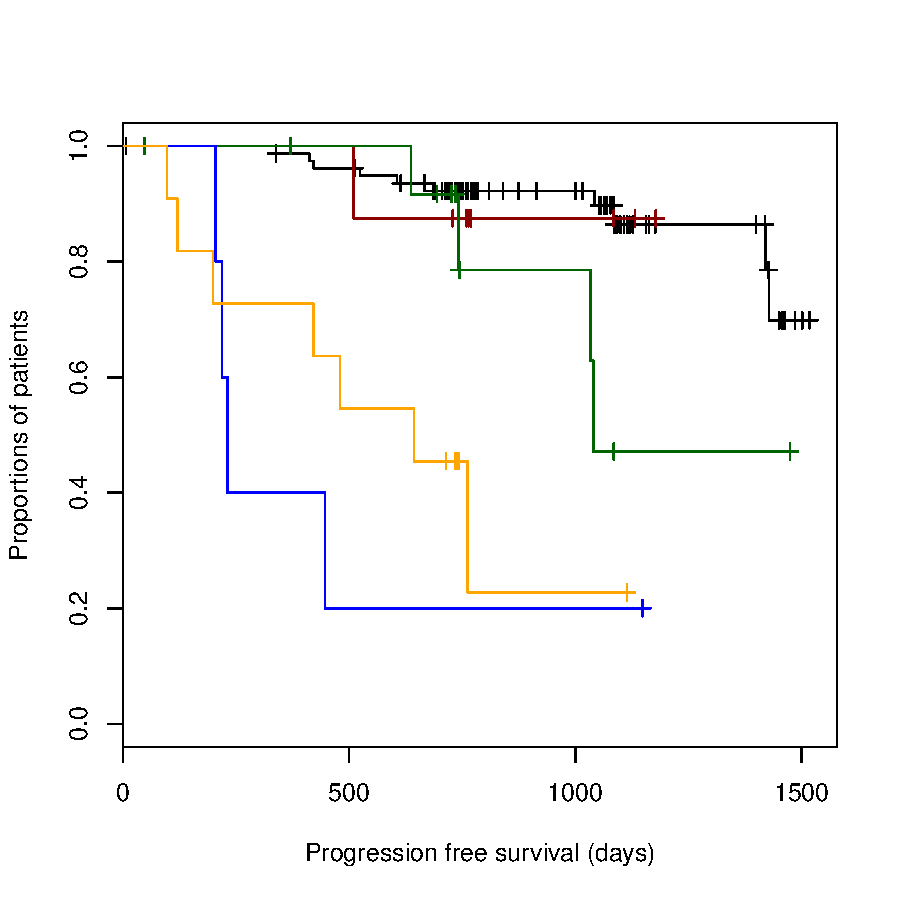
\includegraphics{HICF1_Finalreportv6-033}
\newpage
For TP53\\\
\\
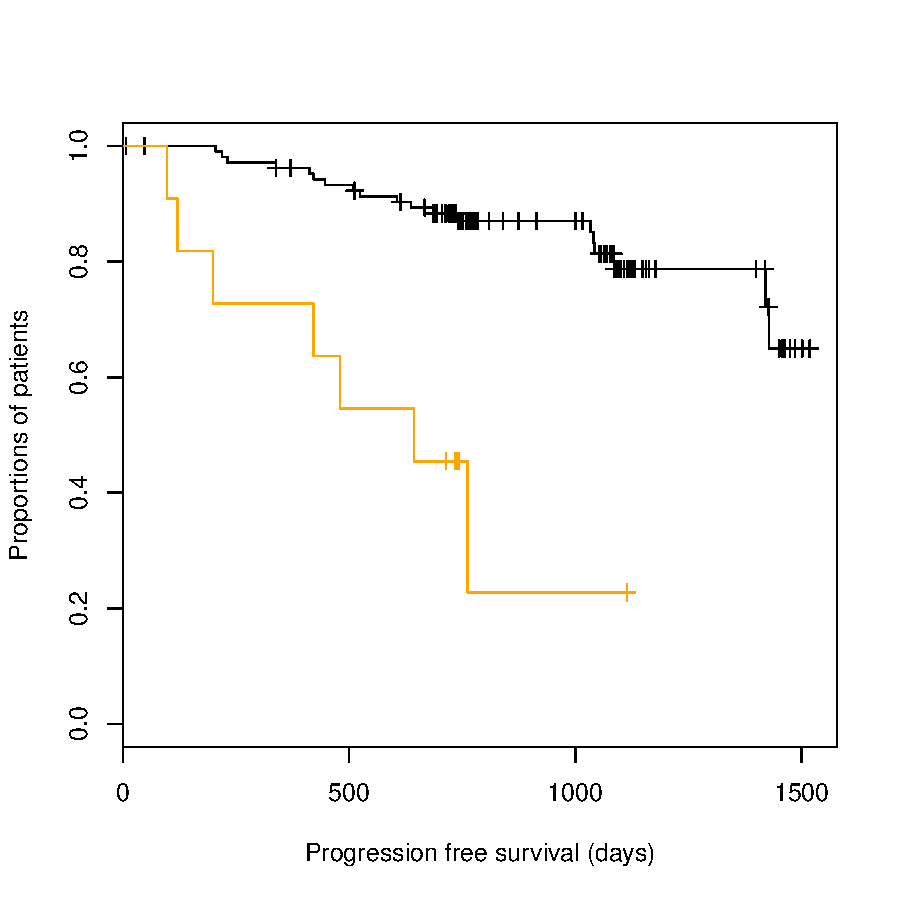
\includegraphics{HICF1_Finalreportv6-035}
\newpage
For SAMHD1\\\
\\
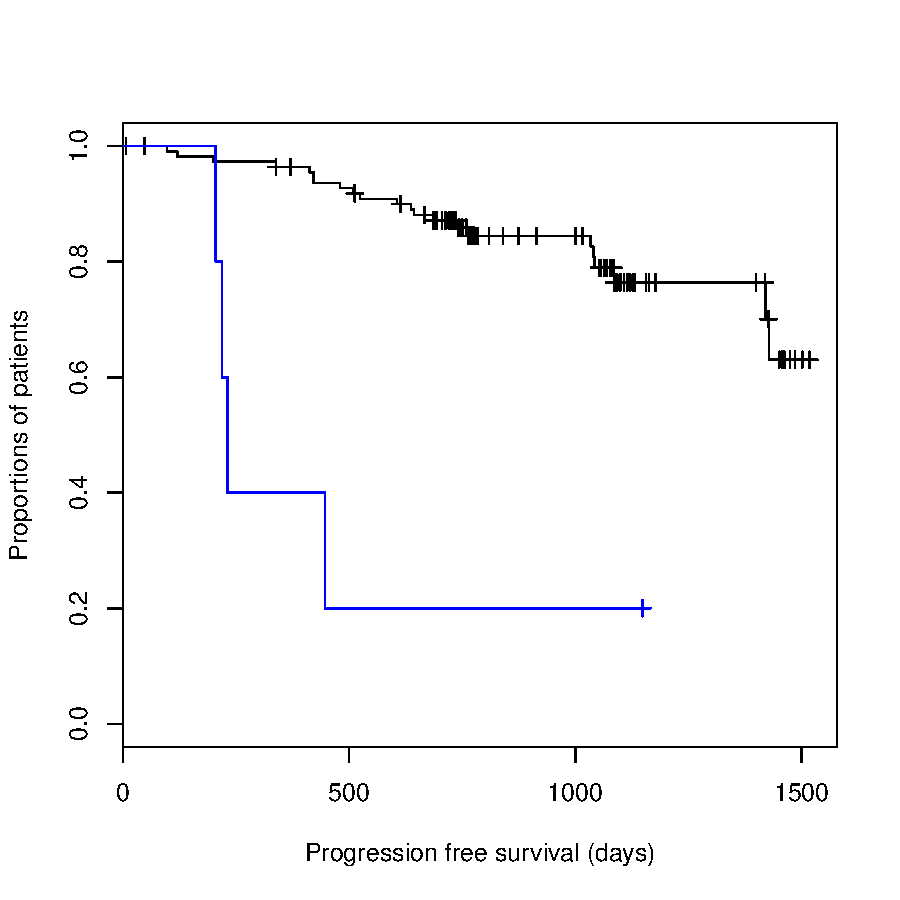
\includegraphics{HICF1_Finalreportv6-037}
\newpage
For Trisomy 12\\\
\\
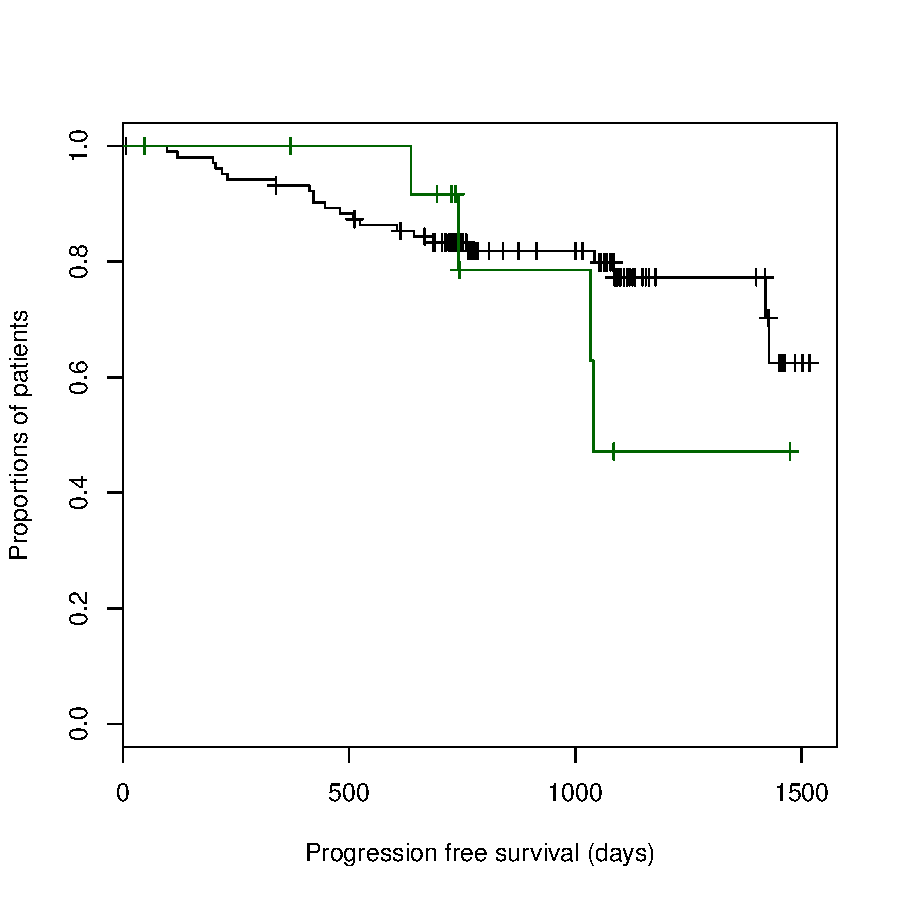
\includegraphics{HICF1_Finalreportv6-039}
\newpage
For ATM bi\\\
\\
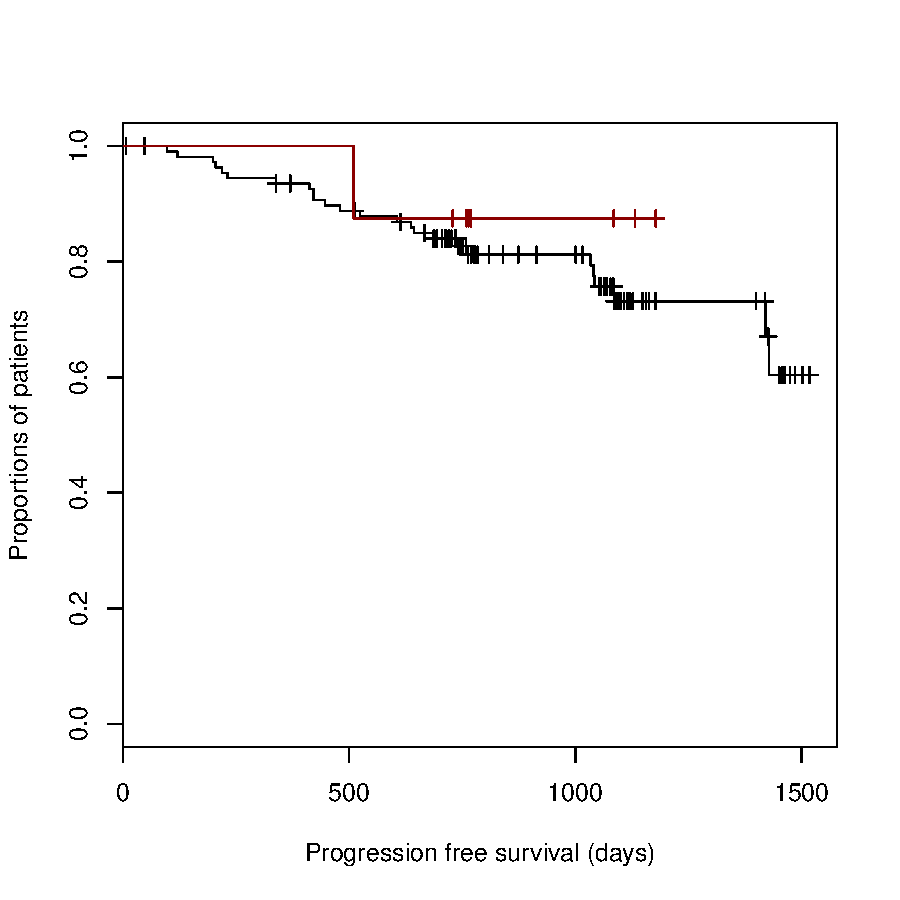
\includegraphics{HICF1_Finalreportv6-041}
\subsection{Logistic regression for patients with survival data}
We can now use the subset of patients for which we have both MRD and PFS data to compare the logistic regression models.\\
The first model uses MRD as response variable and is comparable to the models that we built with the whole data set. The second model uses Progression as response variable. The third model (Combi) uses Progression as response, but includes MRD as predictor.\\
We can see that using MRD as response is fairly unstable and does not give a good prediction with this small data set. Combining both MRD and genetic data however seems to be a very good predictor for progression. Note that we have quite a number of patients with ATM bi that are MRD positive, but did not progress (yet).

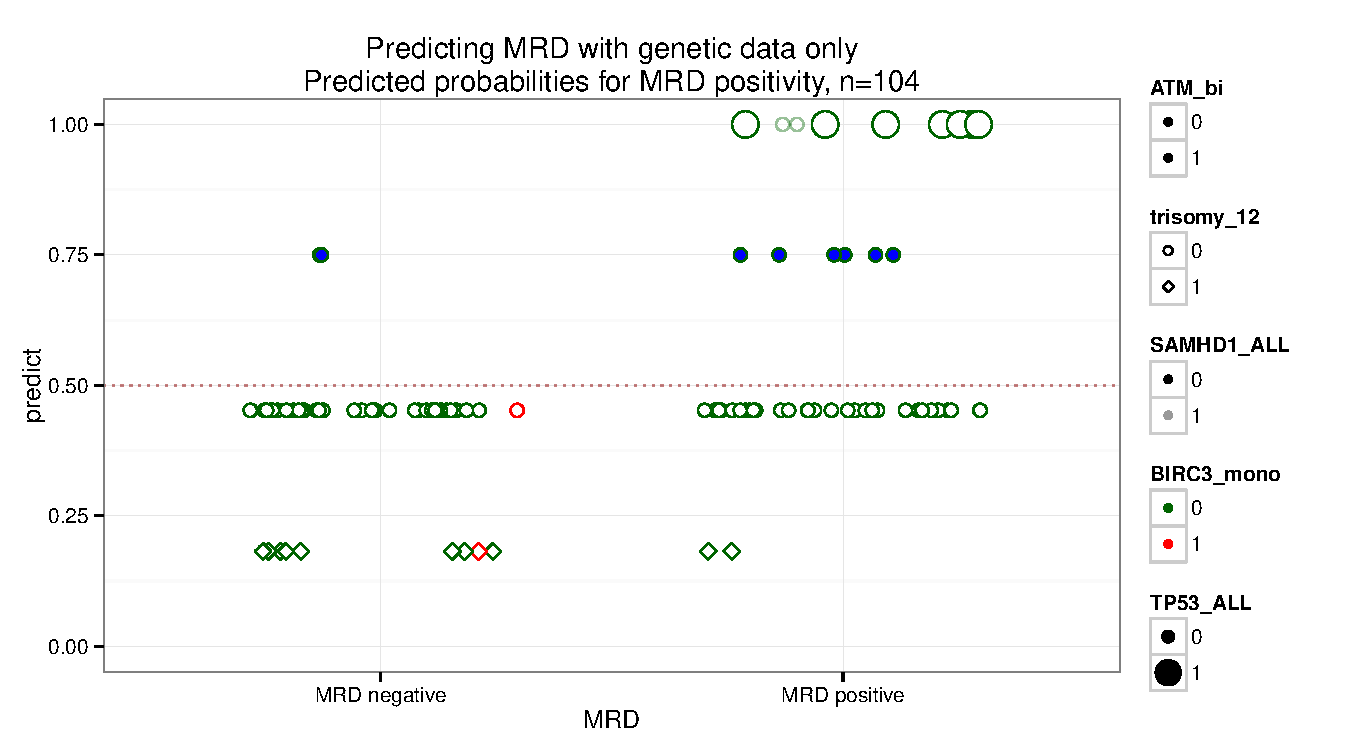
\includegraphics{HICF1_Finalreportv6-043}

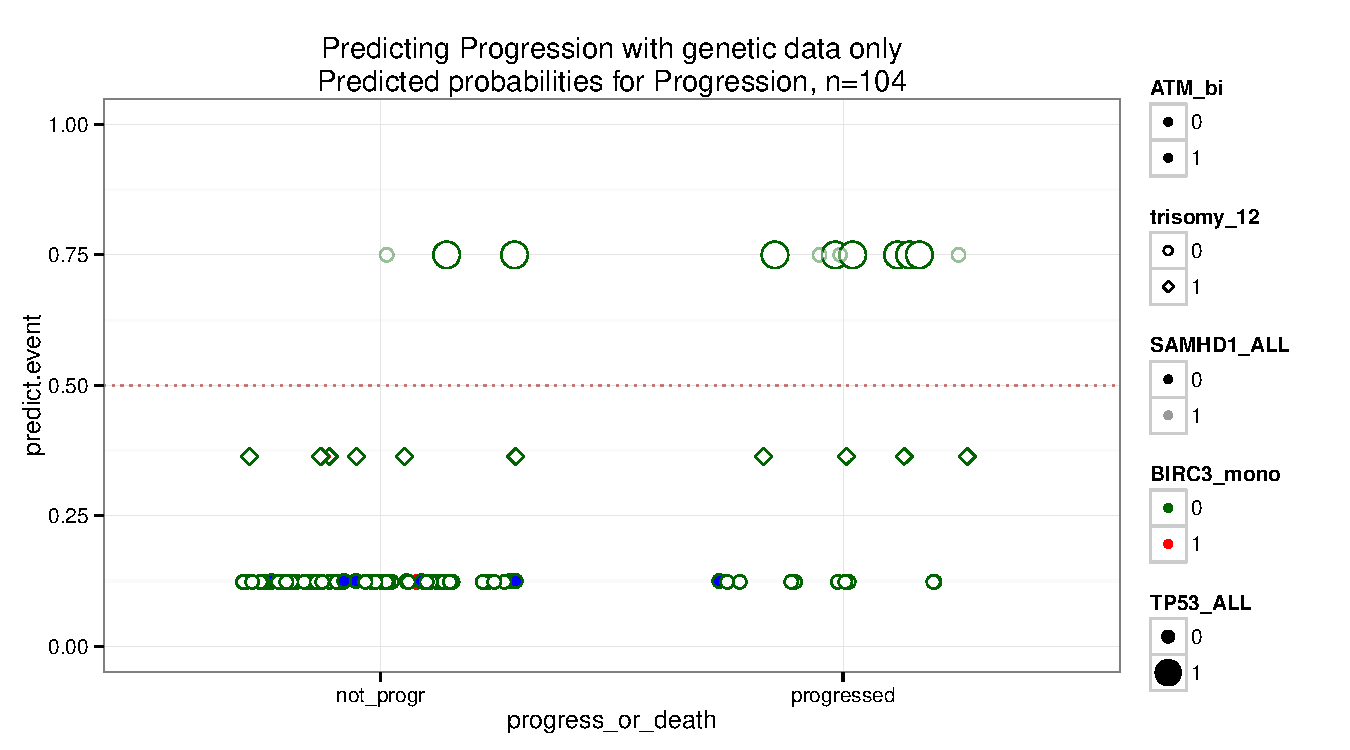
\includegraphics{HICF1_Finalreportv6-044}

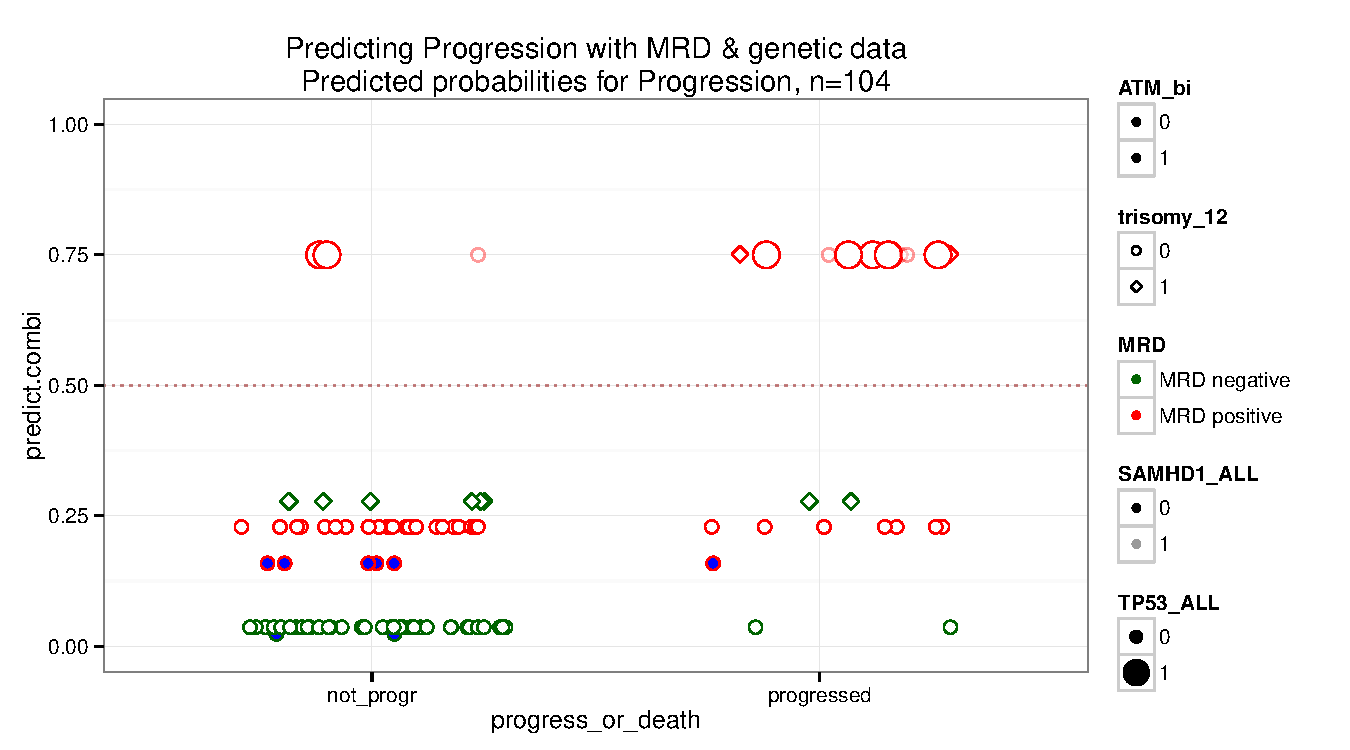
\includegraphics{HICF1_Finalreportv6-045}

% Table created by stargazer v.5.1 by Marek Hlavac, Harvard University. E-mail: hlavac at fas.harvard.edu
% Date and time: Tue, Sep 30, 2014 - 08:53:10
\begin{table}[!htbp] \centering 
  \caption{Compare MRD and Progression Models, n=104} 
  \label{} 
\small 
\begin{tabular}{@{\extracolsep{5pt}}lccc} 
\\[-1.8ex]\hline 
\hline \\[-1.8ex] 
 & \multicolumn{3}{c}{\textit{Dependent variable:}} \\ 
\cline{2-4} 
\\[-1.8ex] & MRD & \multicolumn{2}{c}{progress\_or\_death} \\ 
 & MRD & Progression & Combi \\ 
\hline \\[-1.8ex] 
 TP53\_ALL1 & 17.76 (1,398.72) & 3.06$^{***}$ (0.89) & 2.31$^{**}$ (0.91) \\ 
  ATM\_bi1 & 1.29 (0.85) & 0.02 (1.13) & $-$0.45 (1.15) \\ 
  trisomy\_121 & $-$1.31 (0.82) & 1.40$^{*}$ (0.72) & 2.32$^{**}$ (0.93) \\ 
  SAMHD1\_ALL1 & 17.76 (1,978.09) & 3.06$^{**}$ (1.21) & 2.31$^{*}$ (1.22) \\ 
  MRDMRD positive &  &  & 2.06$^{**}$ (0.82) \\ 
  Constant & $-$0.19 (0.24) & $-$1.96$^{***}$ (0.36) & $-$3.28$^{***}$ (0.76) \\ 
 \hline \\[-1.8ex] 
Observations & 104 & 104 & 104 \\ 
Log Likelihood & $-$59.98 & $-$44.23 & $-$40.03 \\ 
Akaike Inf. Crit. & 129.96 & 98.46 & 92.05 \\ 
\hline 
\hline \\[-1.8ex] 
\textit{Note:}  & \multicolumn{3}{l}{$^{*}$p$<$0.1; $^{**}$p$<$0.05; $^{***}$p$<$0.01} \\ 
\end{tabular} 
\end{table} 

% Table created by stargazer v.5.1 by Marek Hlavac, Harvard University. E-mail: hlavac at fas.harvard.edu
% Date and time: Tue, Sep 30, 2014 - 08:53:10
\begin{table}[!htbp] \centering 
  \caption{Missclassification for pfs models, n=104} 
  \label{} 
\tiny 
\begin{tabular}{@{\extracolsep{1p}} ccccccc} 
\\[-1.8ex]\hline 
\hline \\[-1.8ex] 
 & model & true positive & false positive & true negative & false negative & missclasserr \\ 
\hline \\[-1.8ex] 
1 & fit.survlogreg & $49$ & $35$ & $18$ & $2$ & $0.356$ \\ 
2 & fit.survlogreg.event & $71$ & $13$ & $10$ & $10$ & $0.221$ \\ 
3 & fit.survlogreg.combi & $71$ & $13$ & $10$ & $10$ & $0.221$ \\ 
\hline \\[-1.8ex] 
\end{tabular} 
\end{table} \pagebreak
\section{Patient distributions}
You can use this part of the script to generate a nice distribution of patients by filtering for specific traits first, then ordering by these traits in the order you desire.\\
\begin{center}
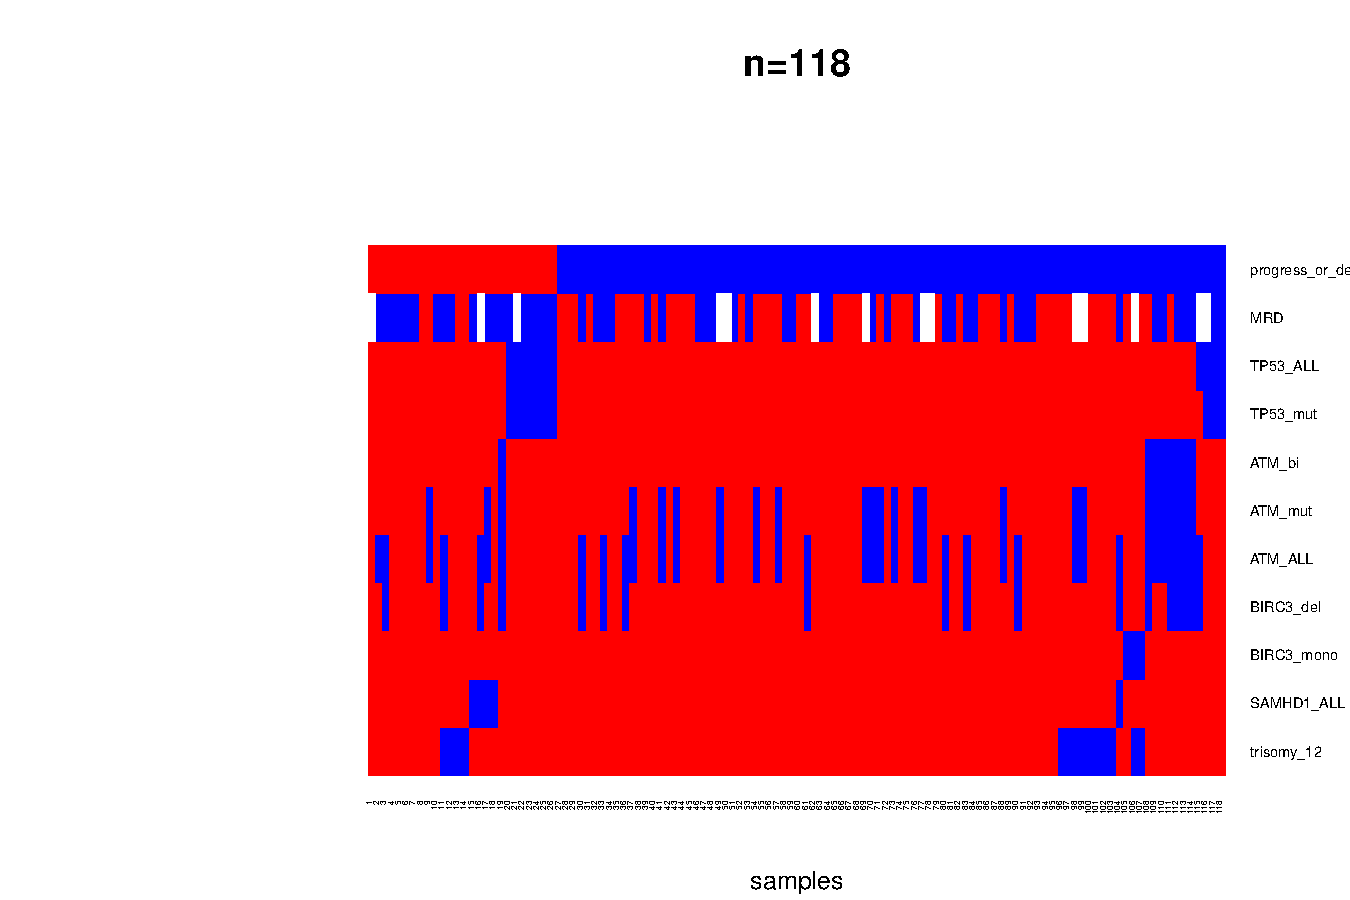
\includegraphics{HICF1_Finalreportv6-049}
\end{center}
\end{document}

